\documentclass[10pt,a4paper,spanish]{report}

\usepackage[spanish]{babel}
\usepackage[utf8]{inputenc}
\usepackage{amsfonts, amssymb, latexsym}
\usepackage{enumerate}
\usepackage[usenames, dvipsnames]{color}
\usepackage{fancyhdr}
\usepackage{geometry}
\usepackage{graphicx}
\usepackage{lastpage}

\definecolor{titlepagecolor}{rgb}{1,0.2,0.3}
\definecolor{namecolor}{rgb}{0.5,1,0.5}

\headsep        3 mm    % space between the head and the body of the page


\usepackage[bookmarks=true,
            bookmarksnumbered=false, % true means bookmarks in
                                     % left window are numbered
            bookmarksopen=false,     % true means only level 1
                                     % are displayed.
            colorlinks=true,
            linkcolor=webblue]{hyperref}
\definecolor{webblue}{rgb}{0, 0, 0.5}  % less intense blue

\pagestyle{fancy}
%con esto nos aseguramos de que las cabeceras de capítulo y de sección vayan en minúsculas

\renewcommand{\sectionmark}[1]{%
      \markright{\thesection\ #1}}
\fancyhf{} %borra cabecera y pie actuales
\fancyhead[LE,RO]{Marta Gómez} % el nombre del autor en la izquierda de las pagibnas pares y a la derecha de las paginas impares
\fancyhead[RE,LO]{\rightmark} % en el lado contrario, la fecha
% PIE DE PAGINA
\fancyfoot[C]{\thepage{} de \pageref{LastPage}}


\usepackage[sfdefault,light]{roboto}  %% Option 'sfdefault' only if the base font of the document is to be sans serif
\usepackage[T1]{fontenc}

%%%%% Para cambiar el tipo de letra en el título de la sección %%%%%%%%%%%
\usepackage{sectsty}
\chapterfont{\fontfamily{frc}\selectfont}
\sectionfont{\fontfamily{frc}\selectfont}
\subsectionfont{\fontfamily{frc}\selectfont}
\subsubsectionfont{\fontfamily{frc}\selectfont}

\setlength{\parindent}{0pt}
\setlength{\parskip}{1ex plus 0.5ex minus 0.2ex}

\begin{document}
\begin{titlepage}
\newgeometry{left=7.5cm} %defines the geometry for the titlepage
\pagecolor{titlepagecolor}
\noindent
% \includegraphics[width=2cm]{logo.jpg}\\[-1em]
\color{white}
\makebox[0pt][l]{\rule{1.3\textwidth}{1pt}}
\par
\noindent
\textbf{\textsf{Gómez Macías}} \textcolor{namecolor}{\textsf{Marta}}
\vfill
\noindent
{\huge \textsf{Fundamentos de bases de datos}}
\vskip\baselineskip
\noindent
\textsf{Febrero-Junio 2015}
\end{titlepage}
\restoregeometry % restores the geometry
\nopagecolor% Use this to restore the color pages to white
% ----------------------------------------------------------------

\thispagestyle{empty}
.\\[175mm]
\begin{center}
\htmladdnormallink{
\includegraphics[width=2cm]{88x31.png}}
{http://creativecommons.org/licenses/by-nc/4.0/}\\
\texttt{Fundamentos de bases de datos by
\href{mailto:mgmacias95@gmail.com}{Marta Gómez Macías}
is licensed under a \htmladdnormallink{Creative Commons
Reconocimiento-NoComercial-CompartirIgual 4.0 Internacional License}
{http://creativecommons.org/licenses/by-nc/4.0/}}.
\end{center}

\tableofcontents

\textcolor[rgb]{1,0.2,0.3}{\chapter{Introducción y definiciones iniciales}}
Antes de existir las bases de datos, se programaban aplicaciones con lenguajes como Cobol que definían una estructura en archivos de registros usando el sistema de archivos como base para el almacenamiento de los datos. Estos programas debían permitir introducir, borrar, modificar y elaborar informes con el contenido de estos archivos.

Los problemas de esta solución son:
\begin{enumerate}[$\heartsuit$]
    \item Los programas dependen de cómo esté estructurado y dónde esté ubicado el fichero. El más mínimo cambio supone cambiar el código del programa.
    \item La información está repetida en varios archivos (redundancia) y da lugar a la inconsistencia de datos.
    \item Seguidad para acceder a los datos, ya que cada tarea puede ser llevada a cabo por un usuario diferente, cada uno debería tener unos permisos sobre los datos.
\end{enumerate}

\textcolor[rgb]{1,0.2,0.3}{\section{Concepto de base de datos y de sistema de gestión de bases de datos}}
Una definición intuitiva de base de datos sería:
\begin{center}
\begin{tabular}{|p{12cm}|}
\hline
\textbf{\textcolor[rgb]{1,0.2,0.3}{Base de datos}}: fondo común de información almacenada en un ordenador para que cualquier persona o programa autorizado acceda a ella independientemente de su procedencia o del uso que vaya a darle.\\
\hline
\end{tabular}
\end{center}

Los elementos de esta definición son:
\begin{enumerate}[$\heartsuit$]
    \item \textcolor[rgb]{1,0.2,0.3}{\textbf{``fondo común de información''}}: implica la posibilidad de compartir información entre usuarios
    \item \textcolor[rgb]{1,0.2,0.3}{\textbf{``almacenada en un ordenador''}}: da carácter de persistencia y determina a la informática como soporte para su implantación
    \item \textcolor[rgb]{1,0.2,0.3}{\textbf{``para que cualquier persona o programa autorizado acceda''}}: refuerza el carácter de información compartida añadiendo el acceso restringido en función de unos privilegios.
    \item \textcolor[rgb]{1,0.2,0.3}{\textbf{``independientemente de su procedencia o del uso que vaya a darle''}}: el lugar y el uso que le dé a la información de la base de datos es ajeno a ésta.
\end{enumerate}

Una definición alternativa sería:
\begin{center}
\begin{tabular}{|p{12cm}|}
\hline
\textcolor[rgb]{1,0.2,0.3}{\textbf{Base de datos}}: una base de datos se compone de una instancia de un \textcolor[rgb]{1,0.2,0.3}{\textit{esquema lógico}} junto a las instancias de datos operativos que dicho esquema organiza. \\
\hline
\end{tabular}
\end{center}

La primera definición se acerca más al concepto de \textit{\textcolor[rgb]{1,0.2,0.3}{sistema de gestión de bases de datos}} y ésta segunda, al concepto de base de datos.

\begin{center}
\begin{tabular}{|p{12cm}|}
\hline
\textcolor[rgb]{1,0.2,0.3}{\textbf{Sistema de gestión de bases de datos}}: conjunto de elementos software con capacidad para definir, mantener y utilizar una base de datos. \\
\hline
\end{tabular}
\end{center}

Las operaciones fundamentales de un sistema de gestión de bases de datos son:

\begin{enumerate}[$\heartsuit$]
    \item Crear, modificar, eliminar y obtener las estructuras asociadas al esquema lógico de la base de datos.
    \item Instanciar datos operativos en una base de datos, modificar las instancias, eliminarlas y recuperarlas con distintos criterios de búsqueda.
\end{enumerate}

\textcolor[rgb]{1,0.2,0.3}{\section{Elementos del concepto de base de datos}}
\textcolor[rgb]{1,0.2,0.3}{\subsection{Los datos}}
Registran el rastro de actividad de la empresa en el sistema. Se deben organizar con un esquema lógico con la info de cada componente de la empresa evitando la redundancia. Debe gestionarse el acceso a los datos de forma que cada usuario acceda a la información que le competa.

\textcolor[rgb]{1,0.2,0.3}{\subsection{El software}}
Hay dos categorías:
\begin{enumerate}[$\heartsuit$]
    \item \textcolor[rgb]{1,0.2,0.3}{\textbf{El sistema de gestión de bases de datos}}: serie de programas que permiten crear, alterar y eliminar bases de datos y que dan al usuario mecanismos para darles contenido y acceder a su información. Disponen de utilidades para garantizar su seguridad y disponibilidad.
    \item \textcolor[rgb]{1,0.2,0.3}{\textbf{Programas de aplicación}}: articulan sobre la base de datos las necesidades de información de los usuarios en base a los requisitos que necesitan.
\end{enumerate}

\textcolor[rgb]{1,0.2,0.3}{\subsection{El Hardware}}
En función de la complejidad del software tendremos arquitecturas más o menos complejas. Desde un esquema Cliente/Servidor en el que el sistema de gestión de datos se ejecuta en el servidor y las aplicaciones en los clientes, hasta arquitecturas distribuidas con varios niveles de ejecución.

\textcolor[rgb]{1,0.2,0.3}{\subsection{Los usuarios}}
En función del uso que hacen del sistema se clasifican en:
\begin{enumerate}[$\heartsuit$]
    \item \textbf{\textcolor[rgb]{1,0.2,0.3}{Terminal (último o final)}}: usa la base de datos para sus actividades, directamente o a través de una aplicación. No necesita conocer cómo se ha implantado ni organizado el sistema.
    \item \textcolor[rgb]{1,0.2,0.3}{\textbf{Programador de aplicaciones}}: desarrolla aplicacionesque den soporte a lo que necesian los usuarios terminales. Necesita recopilar de éstos los requisitos de la aplicación a desarrollar. Interactúa con la base de datos a través de su esquema lógico.
    \item \textcolor[rgb]{1,0.2,0.3}{\textbf{Administrador de la base de datos (\textit{Data Base Administrator})}}: se encarga de la administración del sistema de gestión de bases de datos para que la base de datos cumpla con los requisitos que necesitan aplicaciones y usuarios. También debe garantizar su seguridad y operatividad entre otras cosas.
\end{enumerate}

\textcolor[rgb]{1,0.2,0.3}{\section{Concepto de dato operativo}}
Si consideramos los datos como el concepto fundamental y le vinculamos las operaciones, lograremos mayor flexibilidad. Para ello, debemos establecer el concepto de dato operativo:

\begin{center}
\begin{tabular}{|p{12cm}|}
\hline
\textcolor[rgb]{1,0.2,0.3}{\textbf{Dato operativo}}: todo elemento de información que necesita una organización para su funcionamiento.\\
\hline
\end{tabular}
\end{center}

Hay dos tipos:

\begin{enumerate}[$\heartsuit$]
    \item El \textit{\textcolor[rgb]{1,0.2,0.3}{item básico}} que representa un elemento de información identificable con respecto a los demás.
    \item Los \textit{\textcolor[rgb]{1,0.2,0.3}{vínculos}} entre items básicos.
\end{enumerate}

Se pueden caracterizar mediante \textcolor[rgb]{1,0.2,0.3}{\textbf{atributos}}.

Cuando se identifican y clasifican los datos operativos de una institución se obtiene su \textcolor[rgb]{1,0.2,0.3}{\textit{esquema lógico}}, que representa la estructura de datos de la organización expresada en términos conceptuales. El contenido de dicha estructura, es decir, los datos, se irá generando como consecuencia de la actividad de la organización.

\textcolor[rgb]{1,0.2,0.3}{\section{Independencia de datos}}
El principio de independencia establece el cumplimiento de la siguiente regla fundamental:

\begin{center}
\begin{tabular}{|p{12cm}|}
\hline
Los datos deben organizarse independientemente de las aplicaciones que los vayan a usar y de los ficheros en los que vayan a almacenarse dichos datos. \\
\hline
\end{tabular}
\end{center}

Hay dos niveles de independencia:
\begin{center}
\begin{tabular}{|p{12cm}|}
\hline
\textcolor[rgb]{1,0.2,0.3}{\textbf{Independencia física}}: el almacenamiento físico de los datos debe ser independiente del diseño lógico de la base de datos en todos los niveles.\\
\hline
\end{tabular}
\end{center}

Si cambiamos la estructura física de la base de datos en términos de cambios en los archivos donde se guarda el contenido y en los campos de esos archivos, el esquema lógico de la base de datos debe permanecer inmutable. Así podemos optimizar recursos, cambiar el hardware, etc. Además, hacemos que las aplicaciones se olviden de los problemas físicos.

\begin{center}
\begin{tabular}{|p{12cm}|}
\hline
\textcolor[rgb]{1,0.2,0.3}{\textbf{Independencia lógica}}: la percepción que cada programa tiene de la base de datos debe permanecer inmutable frente a alteraciones a nivel lógico en dicha estructura. \\
\hline
\end{tabular}
\end{center}

Cada programa accede al contenido de la base de datos en función de sus necesidades y privilegios. El sistema de gestión de bases de datos debe proporcionar a cada aplicación su propia perspectiva de la base de datos (vista de usuario).

Un sistema de gestión de bases de datos que mantenga la independencia lógica debe hacer que las vistas de usuario permanezcan inmutables frente a cambios en la estructura lógica de la base de datos. Así, no hará falta modificar el código de las aplicaciones.

\textcolor[rgb]{1,0.2,0.3}{\section{Objetivos de un sistema de gestión de bases de datos}}
\begin{enumerate}[$\heartsuit$]
    \item Garantizar la independencia de los datos
    \item \textcolor[rgb]{1,0.2,0.3}{\textbf{Diseño y utilización orientada al usuario}}: los datos y aplicaciones deben ser accesibles a los usuarios de la manera más amigable posible.
    \item \textcolor[rgb]{1,0.2,0.3}{\textbf{Centralización}}: los datos deben gestionarse de forma centralizada e independiente de las aplicaciones. Un sistema de gestión de bases de datos debe proporcionar herramientas para administrar la base de datos.
    \item \textcolor[rgb]{1,0.2,0.3}{\textbf{Evitar la redundancia y la concurrencia}}: el sistema de gestión de bases de datos debe proporcionar mecanismos para evitar que se dupliquen datos y para gestionar el acceso concurrente de varias aplicaciones a los datos.
    \item \textcolor[rgb]{1,0.2,0.3}{\textbf{Mantener la integridad semántica de los datos}}: la información de la base de datos debe ser siempre correcta. Esto no es posible por:
    \begin{enumerate}[$\longrightarrow$]
        \item \textit{\textcolor[rgb]{1,0.2,0.3}{Seguridad}}: alteración de los datos por parte de un usuario no autorizado
        \item \textcolor[rgb]{1,0.2,0.3}{\textit{Control de recuperación de fallos}}: alteración accidental por un fallo en el sistema.
        \item \textcolor[rgb]{1,0.2,0.3}{\textit{Errores humanos}}: introducción de datos erróneos por parte de un operador autorizado.
    \end{enumerate}
    El sistema de gestión de bases de datos debe proveer mecanismos para evitar las dos primeras. Para evitar la última, debemos establecer los valores que puede tener cada campo (establecer su dominio).
    \item \textcolor[rgb]{1,0.2,0.3}{\textbf{Mantener la fiabilidad del sistema}}: este mecanismo debe acometerse por la implantanción a nivel de almacenamiento, copias de seguridad y redundancia para evitar la pérdida o corrupción de la información.
    \item \textcolor[rgb]{1,0.2,0.3}{\textbf{Mantener la seguridad}}: debemos evitar que usuarios no autorizados accedan a la información no autorizada de la base de datos. Para ello, el sistema de gestión de bases de datos proporciona mecanismos de identificación para definir qué usuario accede a qué recurso.
\end{enumerate}

\textcolor[rgb]{1,0.2,0.3}{\section{Ventajas de la utilización de un sistema de gestión de bases de datos}}
\begin{enumerate}[$\heartsuit$]
    \item Para el usuario:
    \begin{enumerate}[$\longrightarrow$]
        \item \textbf{\textcolor[rgb]{1,0.2,0.3}{Usuario final}}: organizar la información de una empresa mediante una estructura de datos común, accesible y reutilizable por diferentes usuarios y aplicaciones.
        \item \textbf{\textcolor[rgb]{1,0.2,0.3}{Programador de aplicaciones}}: los principios de independencia reducen la necesidad de reescritura de programas frente a cambios estratégicos en los niveles inferiores.
        \item \textcolor[rgb]{1,0.2,0.3}{\textbf{Administrador de la base de datos}}: no existe como usuario.
    \end{enumerate}
    \item Para el sistema:
    \begin{enumerate}[$\longrightarrow$]
        \item Realizar un control centralizado de la información, lo que permite aumentar la integridad de los datos frente a caídas del sistema, reducir la redundancia, incrementar la seguridad, etc.
        \item Criterios de uniformización
        \item Los mecanismos de acceso facilitan el desarrollo de nuevas aplicaciones y la adaptación de las existentes a las necesidades de gestión.
        \item Equilibrio entre requerimientos conflictivos.
    \end{enumerate}
\end{enumerate}

\textcolor[rgb]{1,0.2,0.3}{\chapter{Arquitectura de un sistema de bases de datos}}
\textcolor[rgb]{1,0.2,0.3}{\section{Arquitectura con tres niveles}}
% \textcolor[rgb]{1,0.2,0.3}{\subsection{¿Por qué organizar en niveles?}}
% Los usuarios pueden acceder a los mismos datos, pero desde distintas perspectivas. Si un usuario cambia su forma de verlos datos, no influye en las visiones del resto de usuarios.

% Además, la organización global puede cambiarse sin afectar al resto de usuarios. Y los usuarios no tienen por qué gestionar aspectos relativos a la representación física de los datos. El administrador de la base de datos puede cambiar la forma de representar los datos sin influir en los usuarios.

La arquitectura ANSI/SPARC propugna un modelo de sistema de gestión de bases de datos con tres niveles:

\begin{center}
\begin{tabular}{|p{12cm}|}
\hline
\textcolor[rgb]{1,0.2,0.3}{\textbf{Nivel interno}}: constituye la representación de la base de datos más cercana al nivel físico y es la capa donde se establece la forma en que se implantan las estructuras de datos en las que se organizan los niveles superiores.\\
\hline
\end{tabular}

\begin{tabular}{|p{12cm}|}
\hline
\textcolor[rgb]{1,0.2,0.3}{\textbf{Nivel conceptual}}: supone una visión global de la base de datos que integra todas las visiones que los usuarios tienen de ella.\\
\hline
\end{tabular}

\begin{tabular}{|p{12cm}|}
\hline
\textcolor[rgb]{1,0.2,0.3}{\textbf{Nivel externo}}: define todas las percepciones particulares que tiene cada usuario de la base de datos.\\
\hline
\end{tabular}
\end{center}

La estructura de esta arquitectura sería la siguiente:

\input{arquitectura.latex}

Puede haber varias percepciones externas, pero sólo hay una representación global y una sola implantanción de dicha representación.

Para acotar el significado de nivel externo podemos decir que la percepción de la base de datos de cada usuario se puede plasmar como una estructura de datos.

\textcolor[rgb]{1,0.2,0.3}{\subsection{Nivel externo}}
Cada usuario tiene una percepción de la base de datos llamada visión externa, que está formada por la parte de la base de datos que es relevante para ese usuario y sólo contiene aquellas entidades, relaciones y atributos que le son de interés representados de la forma en la que le interesa. El conjunto de todas las visiones externas forman el nivel externo. La descripción de la vista externa se hace con esquemas externos, para describir sus requisitos usamos DDLs (\textit{\textcolor[rgb]{1,0.2,0.3}{Data Definition Lenguaje}}) en el nivel externo. Estos esquemas se pueden construir a partir del esquema del nivel conceptual o sobre la base de uno o más esquemas externos y constituyen la base de los programas de aplicación. El sistema de gestión de bases de datos debe proporcionar mecanismos para garantizar la inmutabilidad de los esquemas externos frente a cambios en el esquema conceptual.

\textcolor[rgb]{1,0.2,0.3}{\subsection{Nivel conceptual}}
La base de datos es una visión global que integra todas las visiones de los usuarios. Para hacer dicha visión global usamos un DDL a dicho nivel. También podemos implantar restricciones de integridad semántica y reglas de negocio.

El sistema de gestión de bases de datos debe proporcionar un DCL (\textcolor[rgb]{1,0.2,0.3}{\textit{Data Control Lenguaje}}) para implantar políticas de seguridad y restricciones a cada tipo de usuario. 

Este nivel no debe contener ningún detalle sobre el almacenamiento.

\textcolor[rgb]{1,0.2,0.3}{\subsection{Nivel interno}}
% Está formado por una representación abstracta de la estructura de almacenamiento del sistema operativo en el que se ejecuta el sistema de gestión de bases de datos. Esta  representación son archivos organizados según una determinada disposición de campos que almacenan los datos como ocurrencia de registros.

Este nivel es una representación física de la base de datos en el ordenador. Define  cómo están almacenados los datos. Busca el rendimiento óptimo del sistema. Representa estructuras de datos, organizaciones en ficheros, comunicaciones con el sistema operativo para gestionar el uso de unidades de almacenamiento, compresión de datos, encriptación...

Parte de las responsabilidades de este nivel las realiza el sistema operativo

Se debe disponer de un DDL y un DML para definir y acceder a los datos. El DDL debe permitir reestructurar los mecanismos de acceso a la información para mejorar el rendimiento sin que los niveles superiores se vean afectados.

\newpage
\textcolor[rgb]{1,0.2,0.3}{\section{Transformaciones entre niveles}}
Conjunto de normas que establece cómo se define la información de un nivel con respecto de otro. Es esencial para mantener la independencia lógica y física. Hay varios tipos:

\begin{enumerate}[$\heartsuit$]
    \item \textcolor[rgb]{1,0.2,0.3}{\textbf{Transformación conceptual/interno}}: establece la forma en la que se organizan los campos del nivel conceptual en términos de los campos y registros del nivel interno. La independencia física cuando varía el nivel interno hace variar esta correspondencia así, el nivel conceptual no nota dicho cambio.
    \item \textcolor[rgb]{1,0.2,0.3}{\textbf{Transformación externa/conceptual}}: cada esquema externo se define en términos del esquema conceptual. La independencia lógica se consigue modificando dicha correspondencia.
    \item \textcolor[rgb]{1,0.2,0.3}{\textbf{Transformación externa/externa}}: algunos sistemas de gestión de bases de datos permiten describir un esquema externo función de otros esquemas externos. La independencia lógica se mantiene modificando esa correspondencia entre esquemas.
\end{enumerate}

Las correspondencias deben escribirse en un lenguaje inteligible por el sistema de gestión de bases de datos, que suele ser una variante del DSL.  Se recomienda que la base de datos proporcione formas de guardar dichas correspondencias como metainformación para el sistema de gestión de bases de datos.

Las correspondencias externa/conceptual y externa/externa suelen ser descritas por el usuario usando DDL, en cambio, la correspondencia conceptual/interna se suele construir a partir de las definiciones del DBA (\textit{\textcolor[rgb]{1,0.2,0.3}{Data Base Administrator}}) y su construcción suele estar implementada en el sistema de gestión de bases de datos.

\textcolor[rgb]{1,0.2,0.3}{\section{Lenguajes de aplicación y lenguajes de datos}}
La arquitectura ANSI/SPARC recomienda que los sistemas de gestión de bases de datos tengan un lenguaje específico para trabajar: DSL (\textcolor[rgb]{1,0.2,0.3}{\textit{Data SubLenguaje}}). Se subdividen en:

\begin{center}
\begin{tabular}{|p{12cm}|}
\hline
\textcolor[rgb]{1,0.2,0.3}{\textbf{DDL (Data Definition Lenguaje)}}: destinado a la definición de estructuras de datos y esquemas en la base de datos. \\
\hline
\end{tabular}

\begin{tabular}{|p{12cm}|}
\hline
\textcolor[rgb]{1,0.2,0.3}{\textbf{DML (Data Modification Lenguaje)}}: destinado a introducir datos en los esquemas, modificarlos, eliminarlos y consultarlos \\
\hline
\end{tabular}

\begin{tabular}{|p{12cm}|}
\hline
\textcolor[rgb]{1,0.2,0.3}{\textbf{DCL (Data Control Lenguaje)}}: destinado a gestionar los requisitos de acceso a los datos y otras tareas administrativas de la base de datos. \\
\hline
\end{tabular}
\end{center}

La propuesta ANSI/SPARC recomienda tener uno de cada en cada uno de los niveles de la arquitectura. Aunque en la práctica, todos estos sublenguajes se presentan bajo una implementación única en la que todavía es posible distinguir la pertenencia de cada sentencia del lenguaje a cada una de las tres categorías. La separación de los lenguajes en los niveles de la arquitectura se establece con el tipo de sentencias que puede ejecutar cada usuario según sus permisos.

Frente a las recomendaciones de ANSI/SPARC, la industria ha seguido un camino diferente: se ha propiciado la adopción de lenguajes de datos estándar adoptables por diversos fabricantes de sistemas de gestión de bases de datos que no incorporan una separación estricta entre niveles (externo, conceptual, interno) ni de sublenguajes. Un ejemplo destacado son las distintas versiones estandarizadas de SQL.

Los \textit{\textcolor[rgb]{1,0.2,0.3}{lenguajes anfitriones}} son los que sirven para hacer aplicaciones para la base de datos. Pueden ser lenguajes de propósito general (C, Java, Pascal...) o herramientas específicas para bases de datos (Developer de Oracle). Proporcionan procesamiento avanzado de datos y gestión de la interfaz de usuario. Estos lenguajes deben disponer de herramientas para trasladar la estructura de datos del DSL a la estructura de datos propia de cada lenguaje de aplicación e igualmente para las operaciones DSL y las soportadas por cada lenguaje anfitrión. Esta característica se llama \textcolor[rgb]{1,0.2,0.3}{\textit{acoplamiento}} y hay dos categorías:

\begin{enumerate}[$\heartsuit$]
    \item \textcolor[rgb]{1,0.2,0.3}{\textbf{Débilmente acoplados}}: constituidos generalmente por lenguajes de propósito general en los que el programador distingue entre sentencias del lenguaje y sentencias DSL.
    \item \textcolor[rgb]{1,0.2,0.3}{\textbf{Fuertemente acoplados}}: constituidos por las herramientas de propósito específico. El DSL es el elemento central al que se le añaden las características necesarias para desarrollar aplicaciones para bases de datos.
\end{enumerate}

Algunas alternativas para implementar el acoplamiento débil son:

\begin{enumerate}[$\heartsuit$]
    \item \textcolor[rgb]{1,0.2,0.3}{\textbf{Utilización de APIs de acceso a bases de datos}}: el sistema de gestión de bases de datos proporciona una biblioteca binaria y una API para acceder a la base de datos desde el código fuente del programa.
    \item \textcolor[rgb]{1,0.2,0.3}{\textbf{DSL inmerso en el código fuente del lenguaje anfitrión}}: el programador hace un programa híbrido con DSL y lenguaje anfitrión. El sistema de gestión de bases de datos lo traduce en llamadas a su API.
\end{enumerate}

Y, para implementar el acoplamiento fuerte hay varias propuestas (la mayoría propietarias) como PL/SQL de Oracle, que proporciona una extensión procedural para SQL. 

La posibilidad de ejecutar Java a través de una máquina virtual implantada en el propio sistema de gestión de bases de datos añade para algunos sistemas de gestión de bases de datos una estimable capacidad de procesamiento que va más allá de la mera gestión de datos, además de proporcionar una vía estandarizada para compartir y ejecutar código del lado del sistema de gestión de bases de datos.

También han aparecido entornos de desarrollo específicos para el desarrollo de aplicaciones de gestión: diseñadores de informes, diseñadores de formularios, etc.

\newpage
\textcolor[rgb]{1,0.2,0.3}{\section{Enfoques para la arquitectura de un sistema de gestión de bases de datos}}
Inicialmente, toda la carga de gestión y procesamiento recaía en los servidores centrales a los que el usuario accedía a través de terminales. Tanto el sistema de gestión de bases de datos como los programas de aplicación se ejecutaban en el servidor central. 

\begin{center}
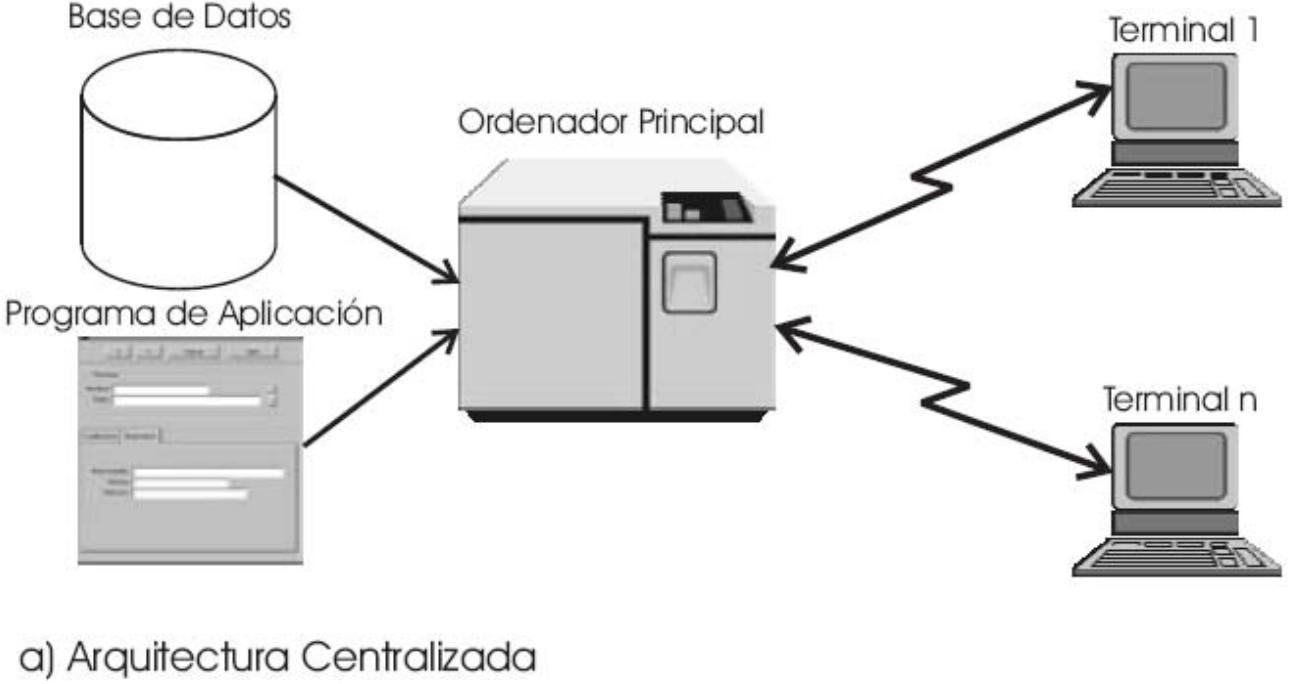
\includegraphics[width=0.6\textwidth]{acentralizada}
\end{center}

El elevado coste de los ordenadores centrales y la aparición de los PCs hizo qye se desplazasen los programas de interacción a los PCs. Lo malo era el mantenimiento de los PCs. La arquitectura Cliente/Servidor en bases de datos hace que el sistema de gestión de bases de datos se divida dos servidores: uno de base de datos y otro que escucha peticiones desde los PCs, que sirve de enlace entre los PCs y la base de datos. En el lado de los PCs, hay programas de aplicación y un enlace que interactúa con el servicio instalado en el servidor.

\begin{center}
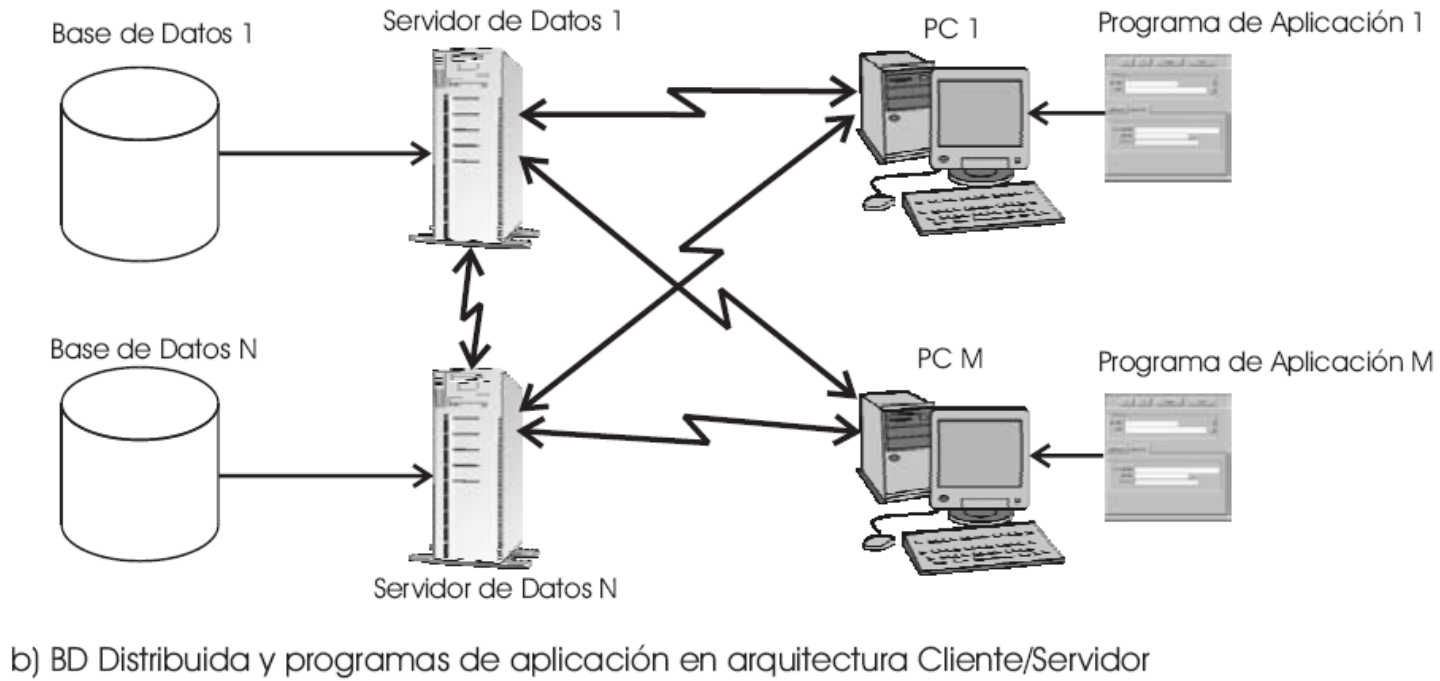
\includegraphics[width=0.6\textwidth]{acs}
\end{center}

Con la aparición de Internet se evolucionó a un enfoque distribuido donde se separan los programas en la parte que interactúa con el usuaro y la parte de ejecución lógica. Así, hay una arquitectura con tres niveles de procesamiento:

\begin{enumerate}[$\heartsuit$]
    \item \textcolor[rgb]{1,0.2,0.3}{\textbf{Nivel de servidor de datos}}: en este nivel podemos organizar una serie de nodos en los que, mediante un sistema de bases de datos distribuido, se gestiona una base de datos distribuida. Este perfil encaja con empresas dispersas que necesitan datos locales y de otras sedes. Los sistemas de gestión de bases de datos distribuidos permiten mantener en una sede copias de los datos de otras sedes así como sincronizarlas. El DBA define la estrategia de copia y sincronización.
    \item \textcolor[rgb]{1,0.2,0.3}{\textbf{Nivel de servidor de aplicaciones}}: el esquema tradicional Cliente/Servidor es muy costoso de mantener para el administrador. Por ello, se propone la utilización se clientes ligeros que disponen de entornos de ejecución estándares y que obtienen las aplicaciones a ejecutar de nodos configurados como servidores. Este esquema requiere de un esfuerzo de configuración y mantenimiento inferior al de cliente/servidor pero precisa de estrategias de administración más sotisficadas y configuraciones redundantes para hardware y software.
    \item \textcolor[rgb]{1,0.2,0.3}{\textbf{Nivel del Cliente}}: en este nivel se dispone de una serie de PCs en los que se reduce la dependencia del hardware y sistema operativo a la hora de abordar la ejecución de aplicaciones.
\end{enumerate}

La ventaja del uso de esta arquitectura reside en la reducción del mantenimiento de los clientes y la mayor facilidad y flexibilidad con la que el usuario  opera con las aplicaciones de las empresa. El inconveniente, la mayor complejidad en la configuración y administración de los servidores de aplicaciones y en el desarrollo de  aplicaciones con el modelo distribuido.

\begin{center}
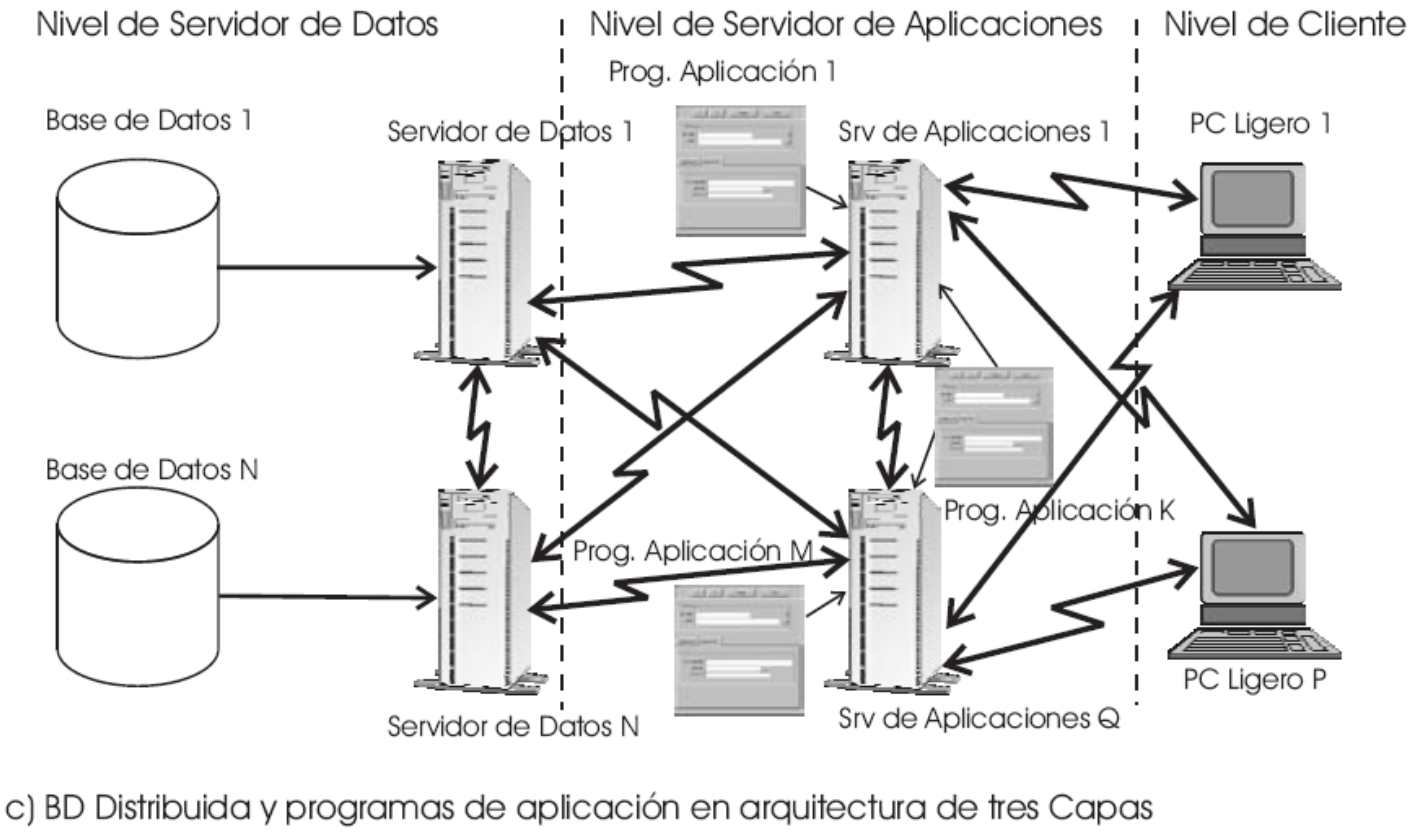
\includegraphics[width=0.6\textwidth]{adistribuida}
\end{center}

\textcolor[rgb]{1,0.2,0.3}{\section{El administrador de la base de datos}}
Sus funciones son:
\begin{enumerate}[$\heartsuit$]
    \item \textcolor[rgb]{1,0.2,0.3}{\textbf{Elaboración del esquema conceptual}}: se desarrolla en estas etapas:
    \begin{enumerate}[1.-]
        \item Análisis de las necesidades de información de la empresa.
        \item Identificación de los datos operativos.
        \item Elaboración del esquema lógico.
        \item Implantación de dicho esquema mediante un DDL.
    \end{enumerate}
    El sistema de gestión de bases de datos almacenará tanto el fuente del esquema como la versión compilada.

    \item \textcolor[rgb]{1,0.2,0.3}{\textbf{Decidir la estructura de almacenamiento en el nivel interno}}: mediante el DDL el DBA define la estructura de almacenamiento y la transformación conceptual/interna. Normalmente, salvo varios aspectos, es el sistema de gestión de bases de datos el encargado de gestionar la transformación.

    \item \textcolor[rgb]{1,0.2,0.3}{\textbf{Conexión con el usuario}}: la visión externa puede ser una visión semántica de una parte de la base de datos o una representación de dicha visión usada por una aplicación. En el primer caso, la base de datos debe recoger esa visión y en el segundo, el administrador debe apotar al programador para hacer la correspondencia externa/conceptual.

    \item \textcolor[rgb]{1,0.2,0.3}{\textbf{Definir las restricciones de integridad}}: tanto las restricciones independientes de la semántica de la nase de datos como las reglas de negocio deben ser recogidas por el DBA en el nivel conceptual.

    \item \textcolor[rgb]{1,0.2,0.3}{\textbf{Definir e implantar la política de seguridad}}: el DBA debe definir qué usuarios pueden acceder a cada parte de la base de datos y con qué nivel de acceso.

    \item \textcolor[rgb]{1,0.2,0.3}{\textbf{Definir e implantar la estrategia de recuperación frente a fallos}}: la caída del sistema o un fallo en uno de sus componentes no puede hacer que se pierdan datos. Por ello, el DBA dispone de varios métodos para prevenir pérdidas de datos (Por ejemplo: el uso de sistemas de gestión de bases de datos redundantes y RAIDs, por si falla una de las unidades que el resto puedan recuperar sus datos) y, debe hacer copias de seguridad periódicas. Los sistemas operativos y los sistemas de gestión de bases de datos ayudan a esta tarea.

    \item \textcolor[rgb]{1,0.2,0.3}{\textbf{Optimización del rendimiento}}: el DBA debe procurar que el sistema de gestión de bases de datos funcione de la manera más eficiente posible, o bien liberando espacio no utilizado y reorganizando las operaciones, o bien añadiendo más recursos.

    \item \textcolor[rgb]{1,0.2,0.3}{\textbf{Monitorizar el sistema de gestión de bases de datos}}: el DBA debe realizar un seguimiento continuo de la actividad de la base de datos para detectar posibles vulneraciones. Los sistemas de gestión de bases de datos proporcinan herramientas para esto.
\end{enumerate}

\textcolor[rgb]{1,0.2,0.3}{\chapter{Modelos de datos}}
Tras obtener un esquema conceptual de nuestro sistema, debemos elegir el modo de implementar dicho esquema en un sistema real. Para ello, haremos un proceso previo de diseño consistente en trasladar las estructuras del esquema a un modelo de datos implementable concreto.

Aquí hay cosas de las transparencias que no sé explicar.

\textcolor[rgb]{1,0.2,0.3}{\section{Modelo jerárquico}}
Fue el primero en implementarse físicamente. Las aplicaciones del nivel externo estaban hechas en Cobol. No se permitía el acceso interactivo a los usuarios, es decir, no existía un lenguaje de consulta.

La estructura de datos básica es un árbol. Hay un nodo ``maestro'' del cual cuelgan el resto de registros llamados secundarios. Por tanto, la base de datos está construida por instancias de árboles de distintos tipos. Funciona bien para relaciones muchos a uno y uno a uno pero debemos duplicar información para plasmar relaciones muchos a muchos. Su estructura es la siguiente:

\input{modjerarquico.latex}

Sus inconvenientes son:
\begin{enumerate}[$\heartsuit$]
    \item El almacenamiento de árboles en fichero es complejo, tenemos que organizar varios tipos de registros en el mismo fichero y mantener punteros entre ellos.
    \item El conjunto de operadores de DML es complicado de implementar y usar.
    \item No se podría insertar ningún registro secundario mientras no exista un registro raíz con el que ``engancharlo''.
    \item La información redundante en las relaciones muchos a muchos hace que la integridad sea difícil de mantener.
\end{enumerate}

\textcolor[rgb]{1,0.2,0.3}{\section{Modelo en red}}
La base de datos está formada por grafos almacenados cuya topología depende de las conexiones existentes entre las entidades. Pueden plasmarse todo tipo de relaciones ya que el modelo implementa las relaciones muchos a muchos.

Los registros son los nodos del grafo y los arcos, los enlaces entre ellos. Las relaciones entre conjuntos de entidades se hacen con \textit{\textcolor[rgb]{1,0.2,0.3}{conectores}}. Su estructura es:

\input{mred.latex}

Tiene una estructura homogénea y es más fácil insertar nuevas entidades en un conjunto, sin embargo, la existencia de enlaces entre registros hace que las operaciones de DDL y DML sean complejas de implementar y usar.

\textcolor[rgb]{1,0.2,0.3}{\section{Modelo relacional}}
Una base de datos está constituida por una serie de tablas llamadas \textit{\textcolor[rgb]{1,0.2,0.3}{relaciones}} que van identificadas por nombre y cuyas filas, llamadas \textcolor[rgb]{1,0.2,0.3}{\textit{tuplas}}, se constituyen de la información de la entidad concreta.

Su estructura sería la siguiente:

\input{mrelacional.latex}

Algunos conceptos iniciales serían:
\begin{enumerate}[$\heartsuit$]
    \item \textbf{\textcolor[rgb]{1,0.2,0.3}{Esquema de una base de datos relacional}}: colección de esquemas de relaciones junto restricciones de integridad.
    \item \textcolor[rgb]{1,0.2,0.3}{\textbf{Instancia de una base de datos}}: colección de instancias de relaciones que verifican las restricciones de integridad
    \item \textcolor[rgb]{1,0.2,0.3}{\textbf{Base de datos relacional}}: instancia de una base de datos junto a su esquema.
\end{enumerate}

\textcolor[rgb]{1,0.2,0.3}{\chapter{El modelo de datos relacional}}
\textcolor[rgb]{1,0.2,0.3}{\section{La estructura del modelo de datos relacional}}
El modelo relacional fue desarrollado por E. F. Cod en 1970. Hasta el final de los 80 se consolidaron todos los aspectos del modelo teórico. SQL es el lenguaje más popular para el manejo de las bases de datos relacionales.

El modelo relacional abarca tres ámbitos distintos:
\begin{enumerate}[$\heartsuit$]
    \item \textcolor[rgb]{1,0.2,0.3}{\textbf{Las estructuras para almacenarlos}}: los datos se estructuran en tablas.
    \item \textcolor[rgb]{1,0.2,0.3}{\textbf{La integridad}}: dichas tablas deben satisfacer unas condiciones que preserven la integridad y coherencia de la información que contienen.
    \item \textcolor[rgb]{1,0.2,0.3}{\textbf{Consulta y manipulación}}: los operadores se aplican sobre tablas y devuelven tablas.
\end{enumerate}

La tabla es la \textit{\textcolor[rgb]{1,0.2,0.3}{estructura lógica}} de un sistema relacional. A nivel físico, se puede almacenar como el sistema considere más adecuado (archivo secuencial, archivo indexado...).

\textcolor[rgb]{1,0.2,0.3}{\subsection{Definiciones iniciales}}
\begin{center}
\begin{tabular}{|p{12cm}|}
\hline
\textcolor[rgb]{1,0.2,0.3}{\textbf{Atributo}}: elemento de información del ``mundo'' que vamos a representar, susceptible de tomar valores. \\
\hline
\end{tabular}
\end{center}

Lo notaremos como $A_i, B_i ; i, j \in \{1,2, \cdots, n\}$

\begin{center}
\begin{tabular}{|p{12cm}|}
\hline
\textcolor[rgb]{1,0.2,0.3}{\textbf{Dominio}}: El dominio $D_i$ es el conjunto de valores que puede tomar el atributo $A_i$. \\
\hline
\end{tabular}
\end{center}

Se suele considerar finito. El dominio de un atributo no coincide con el tipo de dato de dicho atributo cuando se implementa una base de datos relacional.

La mayoría de sistemas de bases de datos no soportan el concepto de dominio y sólo ofrecen tipos de datos. Podemos establecer el dominio de un atributo con reglas de integridad.

\begin{center}
\begin{tabular}{|p{12cm}|}
\hline
\textcolor[rgb]{1,0.2,0.3}{\textbf{Relación}}: Dados los atributos $A_i, i \in \{1, \cdots, n\}$ con dominios asociados $D_i$ (no necesariamente distintos). Definimos la relación asociada a los atributos $A_i, \cdots, A_n$ (que notaremos como $R[A_i, \cdots, A_n]$), como cualquier subjunto finito del producto cartesiano $D_1 \times \cdots \times D_n$. \\
\hline
\end{tabular}
\end{center}

En una relación debemos considerar los siguientes aspectos:
\begin{enumerate}[$\heartsuit$]
    \item \textcolor[rgb]{1,0.2,0.3}{\textbf{Esquema}}: Conjunto de atributos $[A_1, \cdots , A_n]$ junto con sus dominios. Lo notaremos con letras mayúsculas $R, S, \cdots$
    \item \textcolor[rgb]{1,0.2,0.3}{\textbf{Instancia}}: Conjunto de tuplas\footnote{TUPLA: cada una de las filas de la relación} $r = \{t_1, \cdots, t_n\} \subseteq D_1 \times \cdots \times D_n$ que la componen en cada momento. Lo notaremos con letras minúsculas $r, s, \cdots$
\end{enumerate}

El esquema de una relación no varía con el tiempo pero una instancia es siempre variable.

El valor de un atributo $A_j$ para una determinada tupla $t_i$ lo notaremos como $t_i [A_j]$. Si un atributo forma parte de varias relaciones, para distinguir a qué nos referimos lo notaremos como $r.A_j$ si tratamos las instancias o como $R.A_j$ si consideramos relaciones en general.

Se denomina \textcolor[rgb]{1,0.2,0.3}{\textit{Cardinalidad}} de una relación al número de atributos que hay en su esquema: si el esquema tiene $n$ atributos la relación es $n-$aria. El cardinal de una instancia de una relación es el número de tuplas que tiene en cada momento.

\textcolor[rgb]{1,0.2,0.3}{\subsection{Propiedades}}
\begin{center}
\begin{tabular}{p{12cm}}
\hline
Los valores que puede tomar un atributo en una relación son atómicos, en el sentido de que no tienen estructura, son escalares. \\
\hline
\end{tabular}
\end{center}

Esta propiedad no se deriva del concepto de relación. De hecho, es más condición que propiedad. Esta condición se denomina \textit{\textcolor[rgb]{1,0.2,0.3}{condición de normalización}} y las relaciones que la verifican se dice que están en \textcolor[rgb]{1,0.2,0.3}{\textit{Primera Forma Normal}}. Ya que en la definición de dominio no se hace ninguna hipótesis sobre su estructura, de forma adicional se isa esta condición para garantizar la coherencia de las consultas.

Esta condición supone que los valores de los atributos de una relación no pueden ser registros, conjuntos, vectores, otra relación, etc... Por eso, las representaciones basadas en el modelo relacional son extensivas y redundantes.

Como consecuencia de la definición de relación consideramos que tanto la instancia como el esquema de una relación son conjuntos. De esto se derivan las siguientes propiedades:

\begin{center}
\begin{tabular}{p{6cm}}
\hline
No hay orden en las tuplas. \\
\hline
\end{tabular}

\begin{tabular}{p{6cm}}
\hline
No hay orden en los atributos. \\
\hline
\end{tabular}
\end{center}

Una relación puede identificarse con muchas tablas. Por ejemplo, si tenemos una relación $R[A,B,C]$ y una instancia de la misma:

\begin{displaymath}
r = \{(a_1,b_1,c_1), (a_2,b_1,c_2), (a_1,b_2,c_1), (a_2, b_2, c_1), (a_1,b_1,c_2)\}
\end{displaymath}

Las siguientes tablas pueden reflejar la instancia:

\begin{minipage}{0.3\textwidth}
\begin{tabular}{|c c c|}
\hline
$A$ & $B$ & $C$ \\
\hline
$a_1$ & $b_1$ & $c_1$ \\
$a_2$ & $b_1$ & $c_2$ \\
$a_1$ & $b_2$ & $c_1$ \\
$a_2$ & $b_2$ & $c_1$ \\
$a_1$ & $b_1$ & $c_2$ \\
\hline
\end{tabular}
\end{minipage}
\begin{minipage}{0.3\textwidth}
\begin{tabular}{|c c c|}
\hline
$A$ & $B$ & $C$ \\
\hline
$a_2$ & $b_1$ & $c_2$ \\
$a_1$ & $b_1$ & $c_2$ \\
$a_1$ & $b_2$ & $c_1$ \\
$a_2$ & $b_2$ & $c_1$ \\
$a_1$ & $b_1$ & $c_1$ \\
\hline
\end{tabular}
\end{minipage}
\begin{minipage}{0.3\textwidth}
\begin{tabular}{|c c c|}
\hline
$A$ & $C$ & $B$ \\
\hline
$a_2$ & $c_2$ & $b_1$ \\
$a_1$ & $c_2$ & $b_1$ \\
$a_1$ & $c_1$ & $b_2$ \\
$a_2$ & $c_1$ & $b_2$ \\
$a_1$ & $c_1$ & $b_1$ \\
\hline
\end{tabular}
\end{minipage}

El hecho de que no haya orden ni en tuplas ni en atributos determina que para acceder a una tupla, nunca lo haremos a través del valor su fila en la tabla, y, para acceder al valor de un atributo, no lo haremos a través de los valores de su fila y columna.

Otra propiedad derivada del hecho de que una instancia sea un conjunto es:

\begin{center}
\begin{tabular}{p{6cm}}
\hline
No hay tuplas duplicadas. \\
\hline
\end{tabular}
\end{center}

Algunas veces no se conoce el  valor de un atributo para una determinada tupla. En esos casos, a ese atributo de esa tupla se le asiguna un \textit{\textcolor[rgb]{1,0.2,0.3}{valor nulo}}.

En una base de datos relacional, el valor nulo en un atributo puede tener varios siginificados:
\begin{enumerate}[$\heartsuit$]
    \item \textbf{\textcolor[rgb]{1,0.2,0.3}{Valor desconocido}}: se da en el caso de que sepamos que el atributo tiene un determinado valor del dominio pero no sabemos cuál es.
    \item \textcolor[rgb]{1,0.2,0.3}{\textbf{Propiedad inaplicable}}: se da en el caso de que no pueda aparecer un valor porque la propiedad no se da en el sujeto representado por la tupla. Por ejemplo, cuando se intenta dar un valor al atributo \verb*|Nombre-Esposa| a una persona soltera.
\end{enumerate}

En cualquier caso, es un valor más de todos los dominios de la base de datos.

\textcolor[rgb]{1,0.2,0.3}{\section{Integridad relacional}}
\textcolor[rgb]{1,0.2,0.3}{\subsection{Reglas de integridad}}
A diferencia de una instancia, que puede ser considerada un conjunto de instancias de relaciones, el esquema de la base de datos es algo más que un conjunto de esquemas de relaciones ya que está asociado al concepto de \textcolor[rgb]{1,0.2,0.3}{\textit{restricciones de integridad}}.

Las \textcolor[rgb]{1,0.2,0.3}{\textit{restricciones de integridad}} son aquellas restricciones sobre el valor de los atributos que mantienen los datos correctos.

Existen restricciones asociadas a una tabla o atributo, como por ejemplo:

\begin{displaymath}
0 \leq cantidad \leq 120
\end{displaymath}

Pero otras, involucran atributos de otras tablas y se consideran restricciones asociadas a la base de datos. Por ejemplo, no podemos matricular a un alumno inexistente:

\begin{displaymath}
D_{Matricula.DNI} \subseteq D_{Alumnos.DNI}
\end{displaymath}

\textcolor[rgb]{1,0.2,0.3}{\section{Restricciones de integridad}}
Dado que la única forma de caracterizar las tuplas es mediante los valores de sus componentes, necesitamos caracterizarlas mediante éstos:

\begin{center}
\begin{tabular}{|p{12cm}|}
\hline
\textcolor[rgb]{1,0.2,0.3}{\textbf{Clave candidata}}: consideremos una relación $R[A_1, \cdots, A_n]$ y $CC \subseteq \{A_1, \cdots, A_n\}$. $CC$ se denomina clave candidata de $R$ si cumple las siguientes propiedades: \\
1. \textcolor[rgb]{1,0.2,0.3}{\textit{Unicidad}}: $\forall r$, instancia de $R$ y $\forall t_1, t_2 \in r ; t_1[CC] \neq t_2[CC]$ \\
Es decir, para cualquier instancia de $R$, no hay dos tuplas que tengan igual valor para los atributos incluidos en $CC$. \\
2. \textit{\textcolor[rgb]{1,0.2,0.3}{Minimalidad}}: No existe $CC' \subset CC$ tal que verifique 1. \\
\hline
\end{tabular} 
\end{center}

Se denomina \textcolor[rgb]{1,0.2,0.3}{\textit{superclave}} a los conjunto de atributos que verifican sólo la propiedad de unicidad.

En una relación puede haber varias claves candidatas. Denominaremos \textit{\textcolor[rgb]{1,0.2,0.3}{clave primaria}} a una clave candidata elegida por el diseñador.

\begin{center}
\begin{tabular}{p{6cm}}
\hline
El esquema de toda relación incluye una clave primaria.\\
\hline
\end{tabular}
\end{center}

Así, para acceder a una tupla sólo necesitamos dar el valor de su clave primaria. Esta forma de acceder a la información se denomina \textit{\textcolor[rgb]{1,0.2,0.3}{acceso por valor}}.

% \textcolor[rgb]{1,0.2,0.3}{\subsection{Conceptos generales}}
El concepto de integridad se puede aplicar a cualquier base de datos que incluya reglas para mantener correcta la información que almacena. Pero en el modelo relacional, además se mantiene la coherencia de las relaciones y constituyen un elemento clave para configurar la estructura de datos.

En una base de datos podemos encontrarnos dos tipos de reglas:

\begin{center}
\begin{tabular}{|p{12cm}|}
\hline
\textcolor[rgb]{1,0.2,0.3}{\textbf{Reglas específicas}}: provienen de la semántica del atributo y son propias de cada base de datos concreta. \\
\hline
\end{tabular} 

\begin{tabular}{|p{12cm}|}
\hline
\textcolor[rgb]{1,0.2,0.3}{\textbf{Reglas genéricas}}: se aplican a los atributos en función del papel que desempeñañ en la estructura de la base de datos. Por ejemplo, si forman parte de una clave primaria. \\

No son exactamente reglas sino metarreglas, ya que son normas genéricas cuya aplicación en una base de datos concreta genera un conjunto de reglas de integridad. Existen dos reglas de integridad genéricas: regla de integridad de la entidad y regla de integridad referencial.\\
\hline
\end{tabular}
\end{center}

\textcolor[rgb]{1,0.2,0.3}{\subsection{Formulación de las reglas de integridad}}

Las reglas genéricas de entidad giran en torno al concepto de clave primaria y clave externa:

\textcolor[rgb]{1,0.2,0.3}{\subsubsection{La regla de integridad de entidad}}
\begin{center}
\begin{tabular}{|p{12cm}|}
\hline
\textcolor[rgb]{1,0.2,0.3}{\textbf{Integridad de entidad}}: los atributos que forman parte de una clave primaria no pueden tomar valores nulos, ni siquiera parcialmente. \\
\hline
\end{tabular} 
\end{center}

En los atributos que forman parte de la clave primaria, el valor nulo se corresponde con ``valor desconocido''. Si tenemos una clave primaria nula no podríamos identificar totalmente a la tupla a la que corresponde.

\textcolor[rgb]{1,0.2,0.3}{\subsubsection{La regla de entidad referencial}}
Sirve para mantener coherente el estado de la base de datos. Antes de formularla debemos entender el concepto de clave externa:

\begin{center}
\begin{tabular}{|p{12cm}|}
\hline
\textcolor[rgb]{1,0.2,0.3}{\textbf{Clave externa}}: Dadas dos relaciones: $R[A_1, \cdots, A_n]$ con su clave primaria, $CP$ y $S[B_1,\cdots,B_n]$ con $CE \subseteq \{B_1, \cdots, B_n\}$ de manera que $cardinal(CP)=cardinal(CE)$ y los dominios de $CP$ y $CE$ sean concordantes ($\forall A \in CP; \exists B \in CE ~|~ dom(A)=dom(B)$ y viceversa). Decimos que $CE$ es clave externa con respecto a $CP$ si se verifica: \\
$\forall r$ instancia de $R$ y $s$ instancia de $S$, $\forall t \in s \Longrightarrow \exists t' \in r ~|~ t[CE] = t'[CP]$ \\
Es decir, para cualquier pareja de instancias de $R$ y $S$, no puede haber un valor de $CE$ que no exista entre los valores que toma $CP$. \\
\hline
\end{tabular}
\end{center}

En una instancia de una relación, si definimos el \textcolor[rgb]{1,0.2,0.3}{\textit{dominio activo}} de un conjunto de atributos como los valores que toman esos atributos en esa instancia, podemos ver la definición de clave externa de otra manera:

\begin{center}
\begin{tabular}{|p{12cm}|}
\hline
\textcolor[rgb]{1,0.2,0.3}{\textbf{Clave externa}}: Dadas dos relaciones: $R[A_1,\cdots,A_n]$ con su clave primaria $CP$ y $S[B_1,\cdots,B_n]$ con $CE \in \{B_1,\cdots,B_n\}$. Decimos que $CE$ es clave externa con respecto a $CP$ si, $\forall r$, instancia de $R$ y $\forall s$ instancia de $S$, el dominio activo de $CE$ está incluido en el dominio activo de $CP$.\\
\hline
\end{tabular}  
\end{center}

La clave externa puede tomar valores nulos siempre que no se viole otra regla de integridad y la semántica del problema lo permita.

La regla de integridad referencial no es más que la imposición del concepto de clave externa:

\begin{center}
\begin{tabular}{|p{12cm}|}
\hline
\textcolor[rgb]{1,0.2,0.3}{\textbf{Integridad referencial}}: si una relación incluye una clave externa conectada a una clave primaria, el valor de la clave externa debe ser igual a un valor ya existente en el dominio activo de la clave primaria o completamente nulo (si la semántica del problema lo permite).\\
\hline
\end{tabular} 
\end{center}

Puede haber más de una clave externa en una relación y puede haber también una clave externa a la clave primaria de la propia relación.

\textcolor[rgb]{1,0.2,0.3}{\subsection{Mantenimiento de las reglas de integridad}}
Debemos de mantener la integridad de la base de datos porque si no, las entidades pueden llegar a ser indistinguibles y las conexiones del modelo pueden perderse. Por ello debemos tomar ciertas precauciones en los procesos de manipulación de una base de datos (inserción, borrado y actualización).

El encargado de ésto debe ser el sistema de gestión de bases de datos pero muchos sistemas no realizan un seguimiento total de la integridad y debe hacer ésta tarea el DBA con programas adecuados.

\begin{description}
    \item[Para mantener la unicidad de la clave primaria y candidatas]: frente a operaciones de inserción y actualización, el sistema de gestión de bases de datos debe rechazar los valores introducidos que sean iguales a los presentes en la base de datos para los atributos que el diseñador ha definido como clave primaria y claves candidatas. 
    \item[Para mantener la integridad de entidad]: debe comprobarse que el valor de los atributos que forman parte de una clave primaria no es nulo y que ninguno de ellos se repite en procesos de inserción y actualización.
    \item[Para mantener la integridad referencial]:
    \begin{enumerate}[$\heartsuit$]
        \item \textit{\textcolor[rgb]{1,0.2,0.3}{En una inserción}} debe comprobarse que el valor de una clave externa sea nulo (si el diseño lo permite) o concuerde con un valor de la clave primaria de la relación a la que referencia.
        \item \textcolor[rgb]{1,0.2,0.3}{\textit{En una actualización}}:
        \begin{enumerate}[$\longrightarrow$]
            \item Si se actualiza la \textit{\textcolor[rgb]{1,0.2,0.3}{clave externa}} debe comprobarse que se cumplen las condiciones de clave externa
            \item Si se actualiza la \textit{\textcolor[rgb]{1,0.2,0.3}{clave primaria}} deben actualizarse en cadena las claves externas que tomen los valores antiguos de dicha clave primaria o impedir la actualización mientras existan referencias al valor anterior.
        \end{enumerate}
        \item \textcolor[rgb]{1,0.2,0.3}{\textit{En una operación de borrado}}, se deben borrar en cadena las tuplas cuyas claves externas concuerden con la clave primaria de la tupla borrada, o poner a nulo en cadena el valor de la clave externa si las demás restricciones de integridad lo permiten.
    \end{enumerate}
\end{description}

\textcolor[rgb]{1,0.2,0.3}{\chapter{Nivel Interno}}
\textcolor[rgb]{1,0.2,0.3}{\section{Introducción}}
Una característica destacable de un Sistema de Gestión de Bases de Datos es \textit{\textcolor[rgb]{1,0.2,0.3}{almacenar de forma permanente grandes cantidades de datos}}. Y uno de sus principales propósito es \textit{\textcolor[rgb]{1,0.2,0.3}{gestionar de forma eficiente los datos y su almacenamiento}}, lo que implica hacer consultas, modificaciones e inserciones de forma eficiente. La combinación de ambas cosas tiene serias implicaciones sobre la organización lógica y física de los datos.

\begin{center}
\begin{tabular}{|p{12cm}|}
\hline
\textcolor[rgb]{1,0.2,0.3}{\textbf{Nivel interno}}: el nivel interno expresa, en última instancia, las operaciones sobre los datos (creación, alteración y recuperación) en términos de actuación sobre unidades mínimas de almacenamiento denominadas páginas de base de datos. Provee al administrador mecanismos para optimizar el almacenamiento y el acceso a los datos. Se encuentra implementado en el Sistema de Gestión de Bases de datos. \\
\hline
\end{tabular}

\begin{tabular}{|p{12cm}|}
\hline
\textcolor[rgb]{1,0.2,0.3}{\textbf{Nivel físico}}: El nivel físico, que se encuentra implementado en el sistema operativo, proporciona al Sistema de Gestión de Bases de Datos una capa de abstracción sobre el hardware. El nivel interno del Sistema de Gestión de Bases de Datos realiza el acceso a los medios de almacenamiento mediante llamadas a los servicios del sistema de archivos, proporcionado por el sistema operativo. \\
\hline
\end{tabular}
\end{center}

\textcolor[rgb]{1,0.2,0.3}{\section{Dispositivos de almacenamiento}}
Las principales características de los medios de almacenamiento más comunes son:
\begin{enumerate}[$\heartsuit$]
    \item \textit{\textcolor[rgb]{1,0.2,0.3}{Velocidad}}: representa el tiempo de acceso a los datos y se mide en unidades de tiempo.
    \item \textit{\textcolor[rgb]{1,0.2,0.3}{Coste}}: se da en dólares por capacidad de almacenamiento ($\$/Mb$) y representa el coste de adquisión del dispositivo dividido por su capacidad.
    \item \textit{\textcolor[rgb]{1,0.2,0.3}{Capacidad}}: cantidad de datos que es posible almacenar en el dispositivo.
    \item \textit{\textcolor[rgb]{1,0.2,0.3}{Fiabilidad}}: se mide por el tiempo medio entre fallos.
\end{enumerate}

Una clasificación habitual para los medios de almacenamiento es:
\begin{enumerate}[$\heartsuit$]
    \item \textbf{\textcolor[rgb]{1,0.2,0.3}{Almacenamiento primario}}: corresponde a las memorias vivas (memoria caché y memoria principal). Proporcionan la mayor velocidad de acceso, son las más caras y también las que tienen capacidades más limitadas. Son volátiles y pierden la información cuando se corta el suministro eléctrico, por eso, no son adecuadas para contener una base de datos ni considerando un sistema de baterías.

    \item \textbf{\textcolor[rgb]{1,0.2,0.3}{Almacenamiento secundario}}: engloba dispositivos de almacenamiento externo como discos magnéticos. Aunque son 1000 veces más lentos que los dispositivos de almacenamiento primario, tienen mucha capacidad y guardan los datos de forma permanente. Permiten acceso directo a los datos, es decir, podemos recuperar un dato sin leer los anteriores. Son muy adecuados para almacenar bases de datos completas.

    \item \textbf{\textcolor[rgb]{1,0.2,0.3}{Almacenamiento terciario}}: corresponde a los discos ópticos y las cintas magnéticas. Tienen un coste muy bajo y mucha capacidad. El tiempo de acceso a los datos es demasiado grande, sobre todo en cintas magnéticas. Los discos ópticos, que proporcionan acceso directo a los datos, reescritura y están aumentando su capacidad y velocidad de acceso, son una alternativa para guardar copias de seguridad de bases de datos.
\end{enumerate}

En resumen, los Sistemas de Gestión de Bases de Datos utilizan los discos duros como almacenamiento persistente, la memoria caché y la memoria principal para el registro temporal de datos mientras se procesan y las unidades ópticas para la realización de copias de seguridad.

\textcolor[rgb]{1,0.2,0.3}{\subsection{Estructura lógica de los discos duros}}
Los discos duros son los dispositivos usados para el almacenamiento de bases de datos. 

Las unidades de disco duro están constituidas por un conjunto de discos mágneticos colocados en un eje de rotación. Sobre cada una de las caras de los discos hay una cabeza de lectura/escritura que tiene movimiento trasversal. Cuando la unidad está en funcionamiento, todas las caras del disco giran a una velocidad constante. Mediante un mecanismo de posicionamiento muy preciso podemos acceder a cualquier punto de cada cara a través del cabezal para realizar operaciones de lectura o escritura.

Cada cara del disco está compuesta por un conjunto de cilindros concéntricos que a su vez, se dividen en sectores, los cuales representan la unidad mínima de almacenamiento (bloque). Todos los sectores tienen la misma capacidad. 

Para acceder a un sector concreto se debe indicar el cilindro en el que se encuentra, el número de sector dentro del cilindro y cuál de las superficies de los discos lo alberga.

Las unidades de disco suelen disponer de una cache para optimizar sus transferencias E/S.

Los principales parámetros que cualifican una unidad de disco duro son:
\begin{enumerate}[$\heartsuit$]
    \item Capacidad de almacenamiento
    \item Tiempo medio de acceso, que mide el tiempo medio transcurrido entre una instrucción y la obtención de los datos
    \item Velocidad de escritura y lectura ($MB/s$)
    \item Velocidad de rotación (rpm)
\end{enumerate}

Las principales medidas de rendimiento son:
\begin{enumerate}[$\heartsuit$]
    \item \textit{\textcolor[rgb]{1,0.2,0.3}{Tiempo medio de acceso ($ta$)}}: tiempo medio transcurrido entre una instrucción y la obtención de la información.
    \item \textit{\textcolor[rgb]{1,0.2,0.3}{Tiempo medio de búsqueda ($tb$)}}: tiempo medio de posicionamiento en pista
    \item \textit{\textcolor[rgb]{1,0.2,0.3}{Tiempo de latencia rotacional ($tl$)}}: tiempo medio de posicionamiento en sector.

    \begin{displaymath}
    ta = tb + tl
    \end{displaymath}

    \item \textit{\textcolor[rgb]{1,0.2,0.3}{Tiempo medio entre fallos}}
\end{enumerate}

Cuando se implementa el acceso a los datos, las dos cosas que debemos tener en cuenta de un disco duro son:
\begin{enumerate}[$\heartsuit$]
    \item Disponibilidad de acceso directo
    \item El sector representa la unidad mínima de transferencia, porque a nivel del sistema de archivos podemos usar un múltiplo de sectores denominado bloque o página como unidad de E/S.
\end{enumerate}

\textcolor[rgb]{1,0.2,0.3}{\subsection{La memoria principal}}
Es el almacenamiento primario de los computadores. En ella se guardan los datos que necesitan los programas para su ejecución. Un Sistema de Gestión de Bases de Datos lo usa para guardar la porción de base de datos de uso más reciente para acelerar su procesamiento, para almacenar parámetros de estado o el código ejecutable de las sentencias de datos usadas, etc.

Desde el punto de vista del nivel interno, la memoria principal es el elemento intermedio que ubica de forma temporal las operaciones realizadas por el Sistema de Gestión de Bases de Datos, ya que es 1000 veces más rápida que la secundaria pero también es un bien muy preciado (tiene capacidad limitada) y por ello, \textit{\textcolor[rgb]{1,0.2,0.3}{el nivel interno debe optimizar el uso de la memoria disponible para acelerar el procesamiento de los datos}}.

Tanto el disco duro como la memoria principal utilizan distintos niveles de cache para acelerar el acceso a los datos.

\newpage
\textcolor[rgb]{1,0.2,0.3}{\section{Método de acceso a la base de datos}}
Un archivo almacenado se organiza en fragmentos llamados \textit{\textcolor[rgb]{1,0.2,0.3}{páginas de archivo almacenado}}. Cada página puede contener una fracción de registro almacenado o varios registros. A nivel de sistema operativo, cada página está formada por fragmentos llamados \textit{\textcolor[rgb]{1,0.2,0.3}{bloques de SO}}. Un bloque está compuesto por unos determinados sectores de disco:

\begin{center}
\input{disco.latex}
\end{center}

El \textit{\textcolor[rgb]{1,0.2,0.3}{método de acceso}} describe cómo se transforma un registro almacenado en una representación física  a nivel de almacenamiento secundario. 

El acceso a los registros se puede hacer de dos formas:
\begin{enumerate}[$\heartsuit$]
    \item \textcolor[rgb]{1,0.2,0.3}{\textbf{Secuencial}}: recupera todos los registros de un archivo almacenado. Para ello, el Sistema de Gestión de Bases de Datos dispone de una tabla donde relaciona cada archivo almacenado con la dirección de su primera página. A partir de esa primera página el sistema recupera registros de forma secuencial.

    \item \textcolor[rgb]{1,0.2,0.3}{\textbf{Directa}}: recupera únicamente un registro almacenado concreto usando para ello un identificador que ha sido producido como resultado de una operación a nivel conceptual.
\end{enumerate}


El acceso directo se desglosa en los siguientes pasos:

\input{ac.latex}

\begin{enumerate}
    \item El Sistema de Gestión de Bases de Datos proporciona al gestor de archivos la dirección de la página que contiene el registro que ha sido solicitado como resultado de una operación a nivel conceptural o externo
    \item El gestor de archivos del Sistema de Gestión de Bases de Datos pide al Gestor de Disco del sistema operativo los bloques de sistema operativo que integran la página en cuestión.
    \item El gestor de disco determina qué sectores integran las páginas pedid y las solicita a la unidad de disco.
    \item Una vez que el gestor de disco tiene los sectores, los agrupa en bloques y los devuelve al gestor de archivos del Sistema de Gestión de Bases de Datos.
    \item De la página recuperada, el administrador de archivos del Sistema de Gestión de Bases de Datos extrae el registro solicitado.
\end{enumerate}

Para realizar operaciones de inserción, borrado o actualización, el administrador de archivos recupera las páginas involucradas y opera sobre ellas para modificar o incorporar nuevas páginas al archivo almacenado.

Para que el Sistema de Gestión de Bases de Datos pueda localizar el registro almacenado, se usa el \textbf{\textcolor[rgb]{1,0.2,0.3}{RID}} (\textit{\textcolor[rgb]{1,0.2,0.3}{Record IDentifier}}), que es un identificador que almacena el número de página en que se encuentra el registro almacenado y un puntero a una posición que contiene la dirección de comienzo del registro en dicha página. El RID de un registro es el mismo durante toda la existencia de dicho registro.

El RID obecede a la forma en la que los registros se almacenan a nivel físico, por lo que permite acelerar la localización de los registros. Tiene dos partes: la primera indica el número de página donde se encuentra el registro y, la segunda, mediante direccionamiento indirecto indica su posición exacta dentro de la página. Este direccionamiento indirecto es posible gracias a un vector que se encuentra en la cabecera de cada página y que tiene tantas celdas como registros pueden almacenarse en dicha página. Cada celda contiene la dirección lógica del registro, así, los RIDs no tienen que modificarse cuando se desplaza un registro dentro de la página.

\input{rid.latex}

Un registro almacenado tiene una estructura compuesta por una \textit{\textcolor[rgb]{1,0.2,0.3}{cabecera}} donde se describe el número y el tipo de campos almacenados que integran el registro, junto a sus contenidos, es decir, \textit{\textcolor[rgb]{1,0.2,0.3}{datos}}. La extracción de datos de los registros se hace una vez recuperados del almacenamiento secundario.

Las páginas de la base de datos tienen un tamaño múltiplo del tamaño de bloque del sistema operativo\footnote{El tamaño de bloque determina la mínima cantidad de información implicada en una operación E/S}. Para recuperar un registro tendremos que recuperar la página que lo contiene y, por tanto, los bloques que la integran.

Debemos organizar la estructura de almacenamiento y acceso para que en cada operación estén involucradas el menor número de páginas de la base de datos posibles.

\textcolor[rgb]{1,0.2,0.3}{\subsection{El gestor de disco del Sistema Operativo}}
El gestor de disco se encarga de organizar la información que alberga la unidad de disco en términos de conjuntos de bloques donde cada bloque representa un archivo a nivel de sistema operativo. Una base de datos puede valerse de uno o varios archivos para almacenar su contenido. También se encarga de gestionar el espacio libre.

Cada bloque se corresponde con un conjunto de sectores físicos. El gestor de disco conoce y se basa en esta correspondencia para recuperar un bloque solicitado.

Sus funciones más elementales son:
\begin{enumerate}[$\heartsuit$]
    \item Crear un nuevo archivo de sistema operativo
    \item Recuperar un bloque concreto de un determinado archivo de sistema operativo
    \item Reemplazar un bloque por otro en la misma ubicación.
    \item Añadir un nuevo bloque a un conjunto de bloques, lo cual implica incrementar el tamaño del conjunto de bloques y, por tanto, del archivo asociado. Para ello, el gestor de disco debe obtener un bloque libre, asociarlo al conjunto de bloques y devolver la referencia a dicho bloque.
    \item Eliminar un bloque de un conjunto, lo cual implica desvincular dicho bloque de dicho conjunto y asociarlo al conjunto de bloques libres.
    \item Eliminar un archivo de sistema operativo existente, lo cual implica localizar el bloque cabecera del archivo y asociar al conjunto de bloques libres todos los bloques asociados al archivo a eliminar. Por último, se deben borrar todas las referencias al archivo borrado.
\end{enumerate}

\textcolor[rgb]{1,0.2,0.3}{\subsection{El gestor de archivos del Sistema de Gestión de Bases de Datos}}
Se encarga de trasladar representación en términos de campos, registros y archivos almacenados a representaciones en términos de bloques y conjuntos de bloques comprensibles por el gestor de disco del sistema operativo.

Como tenemos que organizar los datos de forma que el tiempo de recuperación sea mínimo, no podemos dejar  que los gestores de disco de los SO implementen la gestión del almacenamiento de la base de datos. Los Sistemas de Gestión de Bases de Datos incorporan sus propios gestores de archivos optimizados y que deben proveer las siguientes funciones:

\begin{enumerate}[$\heartsuit$]
    \item Crear un nuevo archivo almacenado, lo que conlleva asociar al nuevo archivo un conjunto de páginas de la base de datos compuesto al menos por una cabecera que lo identifique.
    \item Eliminar un archivo almacenado
    \item Recuperar un registro almacenado de un archivo almacenado. Normalmente, el Sistema de Gestión de Bases de Datos proporciona el RID del registro para que el gestión de archivos sólo tenga que obtener la página que contiene al registro.
    \item Añadir un nuevo registro a un archivo almacenado. Para ello, el gestor de archivos debe localizar la página más idónea de entre las páginas pertenecientes al archivo para colocar el nuevo registro. Si no hay hueco en ninguna página, se añadiría una nueva página. Finalmente, el gestor de archivos devolvería el RID del nuevo registro.
    \item Eliminar un registro de un archivo almacenado.
    \item Actualizar un registro de un archivo almacenado. Para ello, se recuperará la página que contiene al registro y se sustituirá la información, de no caber en esa página, se pedirá una nueva.
\end{enumerate}

El gestor de archivos organiza la base de datos en un conjunto de archivos de sistema operativo. Cuando crea uno de estos archivos, pide bastante espacio aunque inicialmente no se vaya a ocupar para reducir la fragmentación de disco y el número de peticiones de bloques libres. El gestor de archivos administra internamente este espacio.

El gestor de archivos puede solicitar al gestor de disco más bloques para un archivo de SO determinado con el fin de satisfacer el incremento de sus necesidades de almacenamiento.

La liberación de bloques de un conjunto no se suele dar por cuestiones de reorganización interna

Un conjunto de bloques del SO puede contener a más de un archivo almacenado.

Debemos organizar los registros de un archivo almacenado de forma que el gestor de archivos pueda recuperarlos de forma secuencial. Por tanto, en la cabecera guardaremos la ubicación del primer registro y cada registro debe proporcionar información para acceder al siguiente.

El acceso directo a un registro se hace a través del RID.

\textcolor[rgb]{1,0.2,0.3}{\section{Representación de la base de datos en el nivel interno}}
La representación de la base de datos a nivel conceptual parece reflejar que cada conjunto de registros del mismo tipo es un fichero. Esto no es así, en el nivel interno están todos los registros metidos en el mismo archivo, ya que así es como se consiguen las estructuras más cercanas al almacenamiento a nivel físico de forma que el número de operaciones E/S a la hora de recuperar datos sea mínimo.

En el nivel interno, se tratarán de guardar lo más cerca posible los registros que pertenezcan al mismo conjunto de ítems a nivel conceptual o que pertenezcan al mismo archivo almacenado. Así, podremos recuperarlos todos con unas pocas lecturas de disco.

Existen dos técnicas para agrupar los registros en las páginas del nivel interno:
\begin{enumerate}[$\heartsuit$]
    \item \textcolor[rgb]{1,0.2,0.3}{\textbf{Agrupamiento intra-archivo}}: consiste en ubicar en una misma página registros del mismo tipo. Es la más utilizada y frecuente pues cuando se recupera un registro se suele querer recuperar también sus antecesores y predecesores.
    \item \textcolor[rgb]{1,0.2,0.3}{\textbf{Agrupamiento inter-archivo}}: consiste en ubicar en la misma página registros procedentes de diferentes archivos. Para que esta agrupación sea eficiente debe existir una relación fuerte entre registros de distinto tipo para que su recuperación conjunta sea frecuente. Por ejemplo, almacenar un registros de entidades fuertes junto los registros de las entidades débiles asociadas.
\end{enumerate}

Cada página a nivel interno tendrá por un lado su número de página y, por otro, el número de página de la siguiente página dentro del conjunto de páginas en cuestión. Es decir, si tenemos el archivo almacenado de Profesores en tres páginas, la 3, la 6 y la 7; la primera página tendrá como número de página 3 y como página siguiente 6. La 7, como es la última página, tendrá un puntero nulo (x) como página siguiente indicando que es la última.

Para localizar la primera página de cada conjunto se usa la \textcolor[rgb]{1,0.2,0.3}{\textit{página 0}}. Su finalidad es almacenar, para cada conjunto de páginas, la dirección de su primera página. A partir de ésta, siguiendo las cadenas de punteros, podremos ir recuperando el resto:

\begin{center}
\input{indice.latex}
\end{center}

En general, cada página contendra muchos registros. Los registros se almacenan juntos en la misma página ordenados por su clave y dejando un espacio libre sin ocupar al final. Cuando se llevan a cabo inserciones o borrados, se mantiene el orden lógico dentro de una misma página a base de desplazar, si es necesario, los registros existentes a la hora de ubicar uno nuevo.

% Cada Sistema de Gestión de Bases de Datos puede realizar su propia implementación, la descrita aquí es muy general.

% No existe una relación directa entre fichero almacenado y fichero físico, ya que todos los conjuntos de páginas iran almacenados  en uno o varios ficheros físicos.

\textcolor[rgb]{1,0.2,0.3}{\section{Métodos de organización y acceso a los datos}}
Ningún método de acceso es mejor que otro en términos absolutos, sino que lo serán según el criterio que más prime de acuerdo a los requerimientos del sistema.

La operación más costosa es traerse los datos que se necesiten al búffer realizando accesos a disco, ya que el procesamiento posterior de los datos se puede hacer en memoria principal.

El tiempo de acceso a los datos está dominado por el coste de las operaciones E/S. Así, el número de registros accedidos y el número de bloques consultados es una buena aproximación al tiempo de acceso a los datos. También se debe tener en cuenta la proporción de ocupación de los datos respecto al espacio total requerido para el mantenimiento de la estructura.

Los criterios de evaluación para medir la ``calidad'' de una organización son:

\begin{enumerate}[$\heartsuit$]
    \item \textit{\textcolor[rgb]{1,0.2,0.3}{Tiempo de acceso a los datos}}, medido en número de registros accedidos bajo diferentes condiciones:
    \begin{enumerate}[$\longrightarrow$]
        \item Por \textcolor[rgb]{1,0.2,0.3}{\textit{clave de búsqueda}}: buscar el departamento cuyo código sea 13
        \item Por \textcolor[rgb]{1,0.2,0.3}{\textit{invervalo en la clave de búsqueda}}: buscar los departamentos cuyos códigos están comprendidos entre el 10 y el 25.
    \end{enumerate}
    \item \textcolor[rgb]{1,0.2,0.3}{\textit{Número de accesos a disco en inserciones y borrados}} de datos.
\end{enumerate}

Trabajaremos con dos niveles:
\begin{enumerate}[$\heartsuit$]
    \item Organización de registros de datos a nivel de almacenamiento.
    \item Adición de estructuras complementarias para acelerar el acceso a dichos registros.
\end{enumerate}

\textcolor[rgb]{1,0.2,0.3}{\subsection{Organización secuencial}}
En un fichero de acceso secuencial los registros están almacenados consecutivamente uno detrás de otro en un dispositivo de almacenamiento, así para acceder a un registro en la posición $x$, tendremos que pasar por los $x-1$ registros anteriores.

Si queremos mostrar todos los registros de un fichero, es buena idea que estén todos los registros almacenados conjuntamente. Sin embargo, lo normal es hacer consultas por valor de clave o rango de valores.

\textcolor[rgb]{1,0.2,0.3}{\subsubsection{Proceso de consulta}}
Para hacer una consulta, tenemos que recorrer uno a uno todos los registros del fichero comparando su clave con el valor buscado. En el peor de los casos (o bien el registro deseado es el último de la lista, o bien no está en la lista) el orden de eficiencia de esta operación es $O(n)$. Si no tenemos muchos registros no pasa nada, pero en el momento en el que tengamos una cantidad de datos grande tendremos una pérdida de rendimiento importante.

Los registros están ordenados por una clave llamada \textbf{\textcolor[rgb]{1,0.2,0.3}{clave física}}\footnote{Será la clave por la que se realizará más frecuentemente la búsqueda dentro del fichero de datos, aunque no sea el único campo por el que se puedan realizar consultas}.

La \textcolor[rgb]{1,0.2,0.3}{\textit{operación de inserción}} de un nuevo registro por orden de clave supone, en primer lugar, buscar el sitio que le corresponde. Una vez encontrado, si hay hueco se inserta el nuevo registro y si no, se crea un nuevo bloque o un bloque de desbordamiento.

Es recomendable dejar un hueco al final de cada bloque para no tener que estar haciendo reorganizaciones desde el principio, aunque esto no evita reorganizaciones si la base de datos crece constantemente.

La \textcolor[rgb]{1,0.2,0.3}{\textit{operación de borrado}} de un registro supone, en primer lugar buscar el registro por el valor de su clave y tras el borrado, reorganizar localmente los registros de un bloque.

Esta organización tiene grandes inconvenientes que podrían subsanarse, al menos en parte, mediante el uso de estructuras adicionales para acelerar la localización de los datos y disminuir el número de bloques de disco transferidos.

\begin{center}
\input{secuencial.latex}
\end{center}

\textcolor[rgb]{1,0.2,0.3}{\subsection{Indexación}}
Su objetivo es minimizar el tiempo de acceso a los datos por una clave de búsqueda. Funciona de forma similar al índice de un libro: buscamos en el índice la entrada que indica el número de página que hay que leer. Sus implementaciones más destacadas son:

\textcolor[rgb]{1,0.2,0.3}{\subsubsection{Fichero secuencial indexado - Índices densos}}
Tenemos un fichero secuencial como el que teníamos antes y un \textcolor[rgb]{1,0.2,0.3}{\textbf{fichero índice}} en el que sus registros poseen un campo denominado campo clave y un campo referencia que contiene los RIDS de los registros. La clave física es única, es decir, no hay dos registros con la misma clave. Como índice se considera el campo por el que se ordena el fichero de datos, por eso se les llama \textbf{\textcolor[rgb]{1,0.2,0.3}{índices primarios}}.

\input{fichsecuencial.latex}

Cuando se monta un índice primario sobre un fichero de datos se establece una correspondencia directa entre los valores del campo clave y el registro. Los índices se almacenan por clave, lo cual facilita la búsqueda por clave o rango de valores. Además, los registros del fichero índice (pares clave-RID) son más pequeños que los del fichero de datos, por lo que con una sola lectura de disco habremos traído más registros a memoria y por tanto, haremos las búsquedas más rápido.

Podemos crear diversos índices sobre otros campos que no sean la clave física con los índices \textcolor[rgb]{1,0.2,0.3}{\textbf{secundarios}}. Los registros se mantienen ordenados por este campo y además, puede haber dos registros con el mismo valor.

\input{secundario.latex}

Si se lista el fichero de datos usando el índice secundario, el primer registro a listar podría ser de un bloque y el segundo, de otro bloque distinto y el tecero, del mismo bloque del primero, etc. Lo cual implica que tendremos que hacer muchas más lecturas a disco que con un índice primario donde el orden es el mismo orden físico.

\begin{description}
\item[Proceso de consulta]:


Si hacemos una búsqueda en valor con un índice, sólo tenemos que ir recorriendo el fichero secuencial de índices hasta encontrar el valor deseado. Una vez recuperado el RID del registro tendremos que hacer una lectura adicional a disco para traer el bloque deseado. 

La búsqueda por índice es más rápida que en el fichero de datos. La situación ideal sería poder almacenar todo el fichero de índices en memoria principal. Bajo esta situación la búsqueda del índice no supondría costes de acceso a disco y sólo tendríamos que hacer un acceso a disco para recuperar el bloque del registro.

Si hacemos una búsqueda de un rango de valores, realizamos la búsqueda por valor de la cota inferior del intervalo y, a partir de ahí, iríamos recorriendo cada una de las entradas del índice y recuperando los registros correspondientes con el RID. Si no coindice el RID del registro actual con el bloque del registro anterior se hace una nueva operación E/S. Así hasta encontrarnos con el valor de la cota superior del intervalo.

La \textcolor[rgb]{1,0.2,0.3}{\textit{operación de inserción}} de un nuevo registro, supone por un lado las mismas operaciones que para la inserción en el fichero secuencial y, por otro, insertar la entrada en el índice. Esto se hace igual que la inserción en un fichero secuencial.

Lo mismo puede decirse de la \textcolor[rgb]{1,0.2,0.3}{\textit{operación de borrado}}. Supone por un lado, borrar el registro del fichero de datos y, por otro, borrar su entrada del índice.

Si bien los índices aceleran el acceso a los datos, ralentizan las operaciones de inserción y borrado, ya que debemos mantener el índice. Por ello, antes de crear un índice denso debemos comprobar si su uso está justificado por la frecuencia de las consultas y operaciones de mantenimiento de los datos.
\end{description}

\textcolor[rgb]{1,0.2,0.3}{\subsubsection{Índices no densos}}
En los índices densos hay el mismo número de registros que en los ficheros de datos que indexan, por ello, aunque su tamaño sea menor, siguen siendo demasiado grandes. Para reducir el tamaño de los índices se inventaron los \textcolor[rgb]{1,0.2,0.3}{\textit{índices no densos}}. 

Los índices no densos están compuestos por la clave de búsqueda y la dirección de comienzo del bloque donde puede encontrarse el registro consultable por su valor clave. El número de registros se reduce al número de bloques lo cual hace que el acceso secuencial al índice no denso sea muy rápido.

\input{nodenso.latex}

Existen dos diferencias básicas en la búsqueda en un índice denso y no denso:
\begin{enumerate}[$\heartsuit$]
    \item Una vez encontrado el bloque donde podría hallarse el registro que buscamos(seleccionamos en el índice el valor inmediatamente menor al valor que buscamos), hacemos una  búsqueda secuencial dentro de ese bloque. El único coste que tiene esto es traer el bloque a memoria.
    \item Cuando buscamos un valor en un índice no denso, no podemos asegurar que esté o no esté ese valor hasta que no hayamos consultado el bloque. Es decir, las consultas de tipo existencial pueden resolverse consultando el índice en un índice denso, pero en uno no denso necesitamos de la lectura de bloques de datos.
\end{enumerate}

Los índices no densos sólo pueden definirse sobre la clave física, por tanto, sólo podemos tener un índice no denso por fichero de datos.

Las operaciones de borrado e inserción son menos frecuentes, pues sólo afectan al valor más pequeño de un bloque de datos (el que se encuentra en el índice) o cuando la operación provoca una redistribución de los registros en los bloques de datos.

Se puede montar un índice (denso o no denso) sobre más de un campo de un registro. En ese caso, el valor de la clave en el índice estará formado por la concatenación de los campos indicados. Por ejemplo, podríamos tener el campo \textit{nombre\_alumno} y \textit{dni}: el índice irá bien tanto si buscamos al alumno por su nombre como si lo buscamos por DNI y nombre conjuntamente, pero si hacemos la consulta por el DNI no.

\newpage
\textcolor[rgb]{1,0.2,0.3}{\subsubsection{Índices jerárquicos o índices multinivel}}
Para poder tener todos los índices en memoria principal, y por tanto, tener una lista de índices más pequeña, se planteó hacer índices sobre índices.

Un \textcolor[rgb]{1,0.2,0.3}{\textit{índice multinivel}} está formado por un índice sobre un fichero de datos (primer nivel). Sobre éste índice se crea a su vez un nuevo índice que sería el segundo nivel. Este segundo nivel debe ser un índice no denso, teniendo una sóla entrada por cada bloque del índice de primer nivel. Este proceso puede repetirse sobre cada nivel.

\input{ijerarquico.latex}

Los índices multinivel reducen el número de accesos a disco cuando se busca un registro por valor de la clave de búsqueda del índice. Si tenemos un índice multinivel con $n$ niveles, como mucho realizaremos $n$ accesos a disco (en el caso de tener sólo el índice superior en memoria principal).

Sin embargo, plantea problemas a la hora de hacer inserciones o borrados ya que son ficheros ordenados. Para reducir estos problemas, se suele optar por un índice que deja un espacio en cada entrada para insertar nuevos bloques (\textcolor[rgb]{1,0.2,0.3}{\textit{índice multinivel dinámico}}). Esto se implementa con árboles B y árboles B+.

\textcolor[rgb]{1,0.2,0.3}{\subsubsection{Indexación por árboles B}}
Los árboles-B\footnote{La $B$ proviene de \textit{\textcolor[rgb]{1,0.2,0.3}{balanced}}, equilibrado} son una generalización de los índices multinivel y construyen índices equilibrados. La raíz del árbol es el bloque del nivel superior del índice y las hojas, los bloques del índice de nivel inferior. Al igual que los índices multinivel, su propósito es reducir al máximo las operaciones E/S.

Cada nodo coincide con un bloque de memoria. Las claves contenidas en cada nodo nos llevan hasta el siguiente nodo del nivel inferior y así hasta llegar al bloque del fichero de datos que contiene el registro deseado. Con cada bajada de nivel vamos restringiendo la búsqueda a un subárbol.

\begin{center}
\input{arbol.latex}
\end{center}

Hay dos tipos de nodos:
\begin{enumerate}[$\heartsuit$]
    \item \textcolor[rgb]{1,0.2,0.3}{\textit{Nodos internos}}: constituyen el árbol en sí
    \item \textcolor[rgb]{1,0.2,0.3}{\textit{Nodos hoja}}: reciben el nombre de \textcolor[rgb]{1,0.2,0.3}{\textit{conjunto secuencia}} y proporcionan acceso directo a los registros al ser un índice de primer nivel sobre el fichero de datos.
\end{enumerate}

La estructura de un nodo interno de un árbol de orden $n$ tiene, como mucho $n-1$ valores de clave en el nodo y $n$ punteros $P_i$ que apuntan a un nodo hijo:

\input{estructuraarbol.latex}

Deben cumplirse ciertas restricciones dentro de los nodos:
\begin{enumerate}[$\heartsuit$]
    \item Los valores de las claves ,$C$, están ordenados dentro del nodo: $C_1 < C_2 < \cdots < C_m$ siendo $m <= n-1$
    \item Puede quedar espacio vacío en los nodos, pero los nodos deben estar rellenos hasta la mitad como mínimo
    \item Para todos los valores $x$ del subárbol apuntado por $P_i$ se cumple que $C_{i-1} \leq x < C_i$ excepto para $i=1$ donde $x < C_1$ y $i=m$ donde $x \geq C_m$
\end{enumerate}

La estructura de los nodos hoja está formada por claves $C_i$ ordenadas, referencias $R_i$ a registros del fichero de datos y punteros $P_j$ al siguiente nodo hoja. La lista concatenada de nodos hoja es de gran utilidad al hacer consultas por intervalos.

\input{nodohoja.latex}

Las restricciones en un nodo hoja son:
\begin{enumerate}[$\heartsuit$]
    \item Las claves dentro de un nodo están ordenadas según $C_i < C_j$ para $i < j$
    \item Todas las claves de un nodo han de ser menores que las claves siguientes en el conjunto secuencia
    \item Los nodos han de estar como mínimo rellenos a la mitad
    \item Todos los nodos hoja se encuentran en el mismo nivel, esta restricción da lugar al concepto de árbol equilibrado con el que conseguimos que no haya nodos hoja muy profundos que requieran muchos accesos a disco durante una búsqueda.
\end{enumerate}

\begin{description}
    \item[Proceso de búsqueda]:

    Para buscar un valor, comenzando desde la raíz, se sigue el puntero apropiado. Así, se van comparando los valores hasta llegar  a la entrada del nodo hoja del conjunto secuencia adecuada.

    Para hacer una búsqueda por intervalo, se busca en primer lugar la entrada correspondiente al menor valor del intervalo y después seguir el conjunto secuencia del árbol-B hasta encontrar el valor de la cota superior del intervalo. En cada nodo hoja estará cada RID de cada registro que busquemos por lo que este tipo de consultas es muy eficiente en árboles-B.

    \input{intervalo.latex}

    \item[Operaciones de borrado e inserción]:

    Para eliminar o insertar valores en el árbol sin violar las restricciones anteriores, se usan algoritmos que garantizan que el árbol resultante sea equilibrado. 
\end{description}

\textcolor[rgb]{1,0.2,0.3}{\subsection{Técnicas de acceso directo}}
Las técnicas de acceso directo sirven para acceder a un registro pero, en vez de usar una estructura adicional, se usa un \textcolor[rgb]{1,0.2,0.3}{\textit{algoritmo}} que indique \textcolor[rgb]{1,0.2,0.3}{\textit{directamente}} la posición del registro en cuestión.

\textcolor[rgb]{1,0.2,0.3}{\subsubsection{Ideas básicas acerca del acceso directo}}
Las técnicas de acceso directo consisten en calcular la dirección de un registro mediante la aplicación, a un campo del registro que lo identifique unívocamente, de un algoritmo.

La forma más fácil de diseñar un acceso directo es añadir como campo lógico la dirección que va a tener el registro o una transformación simple de ésta. Por ejemplo, para guardar unas encuestas anónimas, podríamos guardarlas por su orden de llegada y usar este campo para su identificación porque es bastante fácil transformar este campo en una dirección donde situar el registro.

Si no podemos encontrar un campo para identificar unívocamente al registro, podemos usar algún algoritmo que transforme los valores de un cierto campo en una dirección, es decir, en un entero entre 0 y $n$ (siendo $n$ el número total de registros estimados) que sea luego se transformará en un RID:

\input{accesodirecto.latex}

El proceso de direccionamiento transforma la clave física $k$ de un registro en un entero entre 0 y $M$ (siendo $M$ el total de registros que se ha estimado que tendrá el fichero) y usando el valor generado se sitúa al registro en esa posición del fichero. 

Estos algoritmos no suelen mantener el orden de la clave, por lo que a diferencia de la indexación, los registros no están almacenados según su clave física. Por tanto, esta organización no es muy buena para búsquedas por intervalos: una búsqueda por valor se verá muy beneficiada por el uso de estas técnicas mientras que una búsqueda por intervalo se verá muy mermada en rendimiento ya que claves consecutivas pueden estar en bloques distintos.

\newpage
\textcolor[rgb]{1,0.2,0.3}{\subsubsection{Los algoritmos de direccionamiento}}
Si nuestra clave es alfanumérica, el primer paso es transformarla en un valor numérico. Una vez hecho eso, tenemos que asociar a dicha clave un valor entre 0 y $M$. Los algoritmos suelen estar basados en la generación de números pseudo aleatorios, de hecho, cuanta más aletoriedad den, mejor. Los más comunes son:

\begin{enumerate}[$\heartsuit$]
    \item \textcolor[rgb]{1,0.2,0.3}{\textit{Cuadrados centrales}}: se eleva la clave al cuadrado y se eligen tantos dígitos centrales como sea necesario.
    \item \textcolor[rgb]{1,0.2,0.3}{\textit{Congruencias}}: se divide la clave por $M$ y se toma el resto
    \item \textcolor[rgb]{1,0.2,0.3}{\textit{Desplazamiento}}: se superponen adecuadamente los dígitos binarios de la clave y se suman. Muy adecuado para claves alfanuméricas.
    \item \textcolor[rgb]{1,0.2,0.3}{\textit{Conversión de base}}: se cambia el sistema de numeración y se suprimen algunos dígitos resultantes.
\end{enumerate}

\textcolor[rgb]{1,0.2,0.3}{\subsubsection{Problemas del acceso directo}}
Salvo que la clave se diseñe para ello, es muy difícil encontrar una transformación que, aplicada a un determinado campo, dé un entero positivo en el rango $[0,M]$ tal que:

\begin{enumerate}[$\heartsuit$]
    \item No haya dos valores distintos del campo clave que den lugar al mismo número, porque cuando ocurre esto quiere decir que dos registros tienen que ocupar el mismo hueco y, tenemos que buscar una solución para que no se solapen. Cuando se da esta situación decimos que el algoritmo produce \textcolor[rgb]{1,0.2,0.3}{\textit{sinónimos}} o \textcolor[rgb]{1,0.2,0.3}{\textit{colisiones}}.

    \item El algoritmo no produzca muchos ``huecos'', es decir, que no se acumulen todos los valores en un subintervalo de $[0,M]$ dejando ``vacío'' el resto, ya que esto supone que esos mismos ``huecos'' van a aparecer en el espacio asignado al fichero.
\end{enumerate}

Ambos fenómenos están relacionados, porque cuantas más colisiones haya, más se concentrarán las claves generadas en un subintervalo de $[0,M]$.

Para solucionar las colisiones, se suele combinar el acceso directo con una gestión mediante listas de los sinónimos: se asigna al fichero una zona de ``desbordamiento'' y así, cuando se dé una colisión, el registro problemático se almacena en la zona de desbordamiento manteniendo los sinónimos conectados con una lista:

\input{desbo.latex}

Si las claves generadas se concentran mucho y la cantidad de sinónimos se incrementa excesivamente, se hace imposible mantener un sistema de este tipo ya que aparecen muchas listas que mantener y la zona de desbordamiento puede tener un mayor tamaño que la original.

\textcolor[rgb]{1,0.2,0.3}{\subsubsection{El hashing básico o estático}}
La idea de hashing se centra en el siguiente razonamiento: si el problema es que las claves no se distribuyen de manera uniforme, lo que hay que hacer es asignar más espacio a la parte donde aparecen más valores de la clave.

Para realizar una asignación, lo que se hace es dividir el espacio del fichero en ``cubos'' de forma que el algoritmo de direccionamiento sitúa al registro en un cubo y no en una dirección. El algoritmo deberá estar diseñado que ciertos rangos de valores tengan más cubos que otros. Esto se complementa con los ``cubos de desbordamiento'' donde se introducen los registros que no caben en sus respectivos cubos.

Los pasos para insertar un registro serían:
\begin{enumerate}
    \item Transformar su clave
    \item Localizar el cubo que le corresponde
    \item Si hay sitio en el cubo, insertar
    \item Si no, situar el registro en el cubo de desbordamiento y conectarlo con un puntero al cubo que le corresponde
\end{enumerate}

Y los pasos para hacer una búsqueda:
\begin{enumerate}
    \item Transformar la clave
    \item Localizar su cubo
    \item Realizar una búsqueda secuencial dentro del cubo
    \item Si lo encontramos, devolver el registro y terminar
    \item Si no, hacemos un ``barrido por punteros'' a través de los cubos de desbordamiento.
\end{enumerate}

Así, concluímos que los elementos a tener en cuenta a la hora de diselar una organización de hashing son:
\begin{enumerate}[$\heartsuit$]
    \item El número de cubos
    \item El tamaño de los cubos (número de registros por cubo). Hay que tener en cuenta el tamaño de los bloques físicos, lo ideal sería que un acceso a disco nos trajese un cubo.
    \item La transformada clave/dirección, que debe hacer la distribución de la clave por rangos para que unos cubos no se llenen mucho y otros no se queden muy vacíos.
    \item Cuántos y cómo se distribuirán los cubos de desbordamiento.
\end{enumerate}

Un ejemplo de organización por hashing sería:

\begin{center}
\input{hash.latex}
\end{center}

\textcolor[rgb]{1,0.2,0.3}{\subsection{Hashing dinámico}}
El hashing normal sigue teniendo un problema: es necesario conocer la distribución previa de las claves, porque en caso contrario se pueden asignar a un rango de valores menos cubos de los necesarios y aparecen los siguientes problemas:

\begin{enumerate}[$\heartsuit$]
    \item Sigue existiendo riesgo de colisiones
    \item Al aumentar el número de registros, aumentan los registros en páginas de desbordamiento y el tiempo de acceso, porque para acceder tenemos que hacerlo por listas lineales.
    \item Se hacen necesarias las reorganizaciones y cambios en el algoritmo de direccionamiento.
\end{enumerate}

Lo ideal sería no saber de antemano cuántos cubos se necesitarán para cada rango de valores, sino empezar con unos pocos y que se vayan generando de forma dinámica los cubos conforme se vayan necesitando. Esta idea se denomina \textcolor[rgb]{1,0.2,0.3}{\textit{hashing dinámico}} y necesita de una tabla índice como parte del proceso de direccionamiento.

El valor transformado de la clave nos lleva a la entrada de una tabla índice almacenada en memoria; la salida de dicha tabla es la dirección del cubo donde están los registros con ese valor asociado. Inicialmente, varias entradas de la tabla nos llevarán al mismo cubo y conforme se van insertando registros, se van generando nuevos cubos y cambiando las salidas de la tabla índice.

\textcolor[rgb]{1,0.2,0.3}{\subsubsection{Algoritmo de hashing dinámico}}

    Inicialmente tenemos estos datos de partida:
    \begin{enumerate}[$\heartsuit$]
        \item $k$ que es el campo clave física del registro asociado al fichero que vamos a organizar
        \item $k' = h(k)$ es un valor entero $[0,M]$, salida del algoritmo de direccionamiento.
        \item $n$ número de bits que tiene $k'$ en binario
        \item Un valor entero, $d$\footnote{pseudoclave}, tal que $0 < d \leq n$, los $d$ primeros dígitos de $k'$ seleccionarán el cubo, de manera que todos los registros cuyo valor de $k'$ en binario tenga sus $d$ primeros dígitos iguales estarán en el mismo cubo.
        \item Un valor entero $b$ tal que $b < d \leq n$. Inicialmente, el archivo tiene $2^b$ cubos y, como máximo, tendrá $2^d$.
    \end{enumerate}

    El algoritmo consiste en:
    \begin{enumerate}
        \item Se considera una tabla índice en memoria con $2^d$ filas. En la primera columna (valores de campo clave) se sitúan todas las posibles sucesiones de $d$ dígitos binarios. $d$ es la ``profundidad'' de la tabla.
        \item Todas las entradas cuyos $b$ primeros dígitos sean iguales, apuntarán al mismo cubo. Allí se almacenan los registros cuyo valor $k'$ en binario tenga esos $b$ primeros dígitos. La profundidad de los cubos, en principio, es $b$.
        \item Cuando se llena un cubo se parte en dos, poniendo en uno de ellos los registros con el dígito $b+1$ de $k'$ a 0 y en otro los que lo tienen igual a 1. La profundidad local de estos cubos aumenta una unidad.
        \item Si un cubo generado se vuelve a llenar, se divide en dos de nuevo con el mismo proceso, llevando los registros con el dígito $b+2$ igual a cero a un cubo y los que lo tienen a 1 al otro. La profundidad local de estos cubos sería $b+2$.
    \end{enumerate}

En la siguiente imagen tenemos un ejemplo donde $d = 4$ y $b=2$. Inicialmente, las 16 filas de la tabla índice auxiliar se han dividido en grupos de 4, y cada grupo apunta a un cubo. Posteriormente, se van generando nuevos cubos de forma que hay zonas  de la tabla donde cada fila apunta a un cubo y otras en las que se mantiene el esquema inicial. En cada cubo se indica la profundidad local.

\input{hdin.latex}

El inconveniente del hashing dinámico es el tener que usar una tabla adicional, lo que podría requerir más accesos a disco si la tabla no estuviese en memoria mientras se trabajase con el fichero. Pero como el tamaño de la tabla depende de $d$, ajustando $b$ y $d$ de manera adecuada la tabla puede caber en memoria principal.

\textcolor[rgb]{1,0.2,0.3}{\subsection{Otras técnicas: estructuras multilista}}
La organización encadenada o con estructuras multilista se orientó inicialmente a permitir el acceso según el valor de otros campos que no fuesen la clave física. Su idea básica es:

\begin{center}
\begin{tabular}{p{12.5cm}}
\hline
Se construyen listas lineales enlazando aquellos registros que tienen el mismo valor en el campo clave y el sistema se complementa con un fichero adicional donde se recogen los valores de la clave convenientemente ordeados y conectados con el principio y el final de su lista. \\
\hline
\end{tabular}
\end{center}

Por ejemplo, si tenemos la siguiente base de datos:

\begin{center}
\begin{tabular}{c c c c}
\hline
Código & Nombre & Nivel & Ciudad \\
\hline
S1 & Pérez & Muy alto & Atenas \\
S2 & López & Bajo & Londres \\
S3 & Ruiz & Medio & Londres \\
S4 & Díaz & Alto & Atenas \\
S5 & Paz & Muy alto & París \\
S6 & Vila & Muy alto & Londres \\
\hline
\end{tabular}
\end{center}

Y queremos recuperar la información por los campos ciudad y nivel (siendo el Código la clave física). Montamos la siguiente organización multilista:

\input{multilista.latex}

Los posibles campos para los que se ha montado la estructura de acceso encadenado generan dos ficheros donde se almacenan sus posibles valores. Para recuperar los registros tenemos que entrar en el fichero correspondiente, localizar el campo que queremos recuperar (en el ejemplo están ordenados para hacer una búsqueda) y a partir de él, seguir la lista de punteros.

Estas estructuras se denominan ``padre/hijo'', considerando al padre como el archivo con los valores clave. Se puede montar una estructura con más de un ``padre'' para el mismo archivo ``hijo''.

\textcolor[rgb]{1,0.2,0.3}{\subsubsection{Ventajas e inconvenientes de la organización encadenada}}
\begin{description}
    \item[Ventajas]:

    \begin{enumerate}[$\heartsuit$]
        \item Es muy eficaz para acceder según los valores del campo clave. Con una buena estructura de agrupamiento, es de los más rápidos
        \item Ocupa menos memoria que una tabla índice porque los datos aparecen una sola vez. Elimina redundancia y facilita las operaciones de actualización
    \end{enumerate}

    \item[Inconvenientes]:

    \begin{enumerate}[$\heartsuit$]
        \item Cuando se desea obtener la información del ``padre'' a partir del ``hijo'', el acceso es muy costoso ya que, por ejemplo, si queremos la información del registro con código S1 tendremos que:
        \begin{enumerate}[1.]
            \item Localizar el registro dentro del fichero
            \item Para conocer la ciudad, movernos por los punteros a través de los registros S3 y S4 hasta llegar a ``Atenas''
            \item Y para el nivel, lo mismo, pero está vez con tres registros (S4, S5 y S6) para llegar hasta ``Muy alto''.
        \end{enumerate}
        \item Al haber tantos punteros implicados y ser tan compleja, su mantenimiento suele ser complicado
        \item Tenemos que tener un sistema de acceso alternativo para todos los ficheros, pues el proceso siempre empieza con un acceso al fichero ``padre'' o al fichero ``hijo''.
    \end{enumerate}

    \item[Formas de evitar los inconvenientes]:

    \begin{enumerate}[$\heartsuit$]
        \item Utilizar cadenas de punteros dobles y así reducir el proceso de búsqueda a través de los registros ``hijos'' a la mitad.
        \item Mantener los registros completos en el fichero ``hijo'' para que los accesos ``hijo/padre'' sean innecesarios.
    \end{enumerate}
\end{description}

\textcolor[rgb]{1,0.2,0.3}{\subsubsection{La estructura multilista y la conexión entre ficheros}}
La verdadera utilidad de las multilistas es conectar ficheros a través de un campo común, la de acceder a registros por campos que no es su clave está ya resuelto con la indexación por claves secundarias y con menos esfuerzo y complejidad.

Si el fichero ``hijo'' incluye un campo que referencia a los registros del ``padre'', tenemos dos ficheros conectados a través de dicho campo. Por ejemplo, si en el ejemplo anterior guardamos información adicional sobre cada ciudad, podríamos resolver consultas tales como ``obtener todos los vendedores que están en ciudades con más de 100.000 habitantes''.

Esto muestra cómo podemos reflejar algunas características del concepto de base de datos: conectar distintos ficheros de forma que la información se almacene sin redundancia y se pueda recuperar moviéndonos a través de los mismos.

\end{document}
\textcolor[rgb]{1,0.2,0.3}